%\subsection{Fonction d’onde dans le secteur ordonné et représentation de Gaudin}
%%Dans ce chapitre, nous nous intéressons aux fluctuations de la distribution de rapidité \( \delta \rho \) autour d'une distribution de référence \( \rho^c \), qui maximise la contribution à la fonction de partition des états, exprimée comme une fonctionnelle de la distribution \( \rho \) : 

La fonction de partition des états, s'exprime comme une fonctionnelle de la distribution \( \rho \) : 

\begin{eqnarray*}
	\Xi & = & \sum_\rho \exp \left( -\mathcal{A}(\rho) \right).
\end{eqnarray*}  

Dans la section {\em \bf Entropie de Yang-Yang} (\ref{??}), l'action \( \mathcal{A}(\rho) \) s'écrit sous la forme :  

\begin{eqnarray*}
	\mathcal{A}(\rho) & \doteq & - L\mathcal{S}_{YY}(\rho) + L\int f(\theta) \rho (\theta) \, d\theta,		
\end{eqnarray*}  

où \( \mathcal{S}_{YY} \) est la fonctionnelle d'entropie de Yang-Yang, définie dans (\ref{??}), et \( f \) est la fonction paramétrant les charges, introduite dans (\ref{??}).  

Dans cette même section {\em \bf Entropie de Yang-Yang} (\ref{??}), nous avons établi un lien entre \( f \) et distribution de référence \( \rho^c \), qui maximise la contribution à la fonction de partition des états .\\

On veux tester si nos experience est décrit pas un GGE. Pour cela nous nous intéressons aux fluctuations de la distribution de rapidité \( \delta \rho \) autour \( \rho^c \).

%Nous poursuivons à présent avec cette définition de l'action de classe $\mathcal{C}^2$ et admetant une distribution critique $\rho^c$ tel que sa différentielle en ce point critique soit nulle $d\mathcal{A}_{\rho^c} = 0 $ (\ref{??}) de sorte que d'aprés la formule de Taylor-Youg %afin de déterminer les fluctuations autour de \( \Pi^c \). Pour cela, nous réécrivons l'action sous la forme :  

Nous poursuivons à présent avec cette définition de l'action de classe $\mathcal{C}^2$ et admetant une distribution critique $\rho^c$ tel que sa différentielle en ce point critique soit nulle $d\mathcal{A}_{\rho^c} = 0 $ (\ref{??}) de sorte que d'aprés la formule de Taylor-Youg %afin de déterminer les fluctuations autour de \( \Pi^c \). Pour cela, nous réécrivons l'action sous la forme :  

\begin{eqnarray*}  
	\mathcal{A}(\rho^c + \delta \rho) & \underset{ \delta \rho \to 0 }{=} & \mathcal{A}(\rho^c)  + \frac{1}{2} \left. \frac{\delta^2 \mathcal{A}}{\delta \rho^2} \right|_{\rho^c} (\delta \rho) + \mathcal{O}((\delta \rho)^3),  
\end{eqnarray*}  

une expression quadratique pour l'action à l'ordre dominant en \( \delta \Pi \) avec $\left. \frac{\delta^2 \mathcal{A}}{\delta \rho^2} \right|_{\rho^c}$ la forme quadratique définie positive (Fig (\ref{fig.fluctu.A})).

\begin{figure}[H]
	\centering 
	\begin{tikzpicture}
		\begin{scope}[shift={(0,0)}]
			\begin{scope}[transform canvas={scale=0.6}]
				% Définition des couleurs avec les codes HTML
\definecolor{colorOne}{HTML}{443E46}
\definecolor{colorTwo}{HTML}{F6DEB8}
\definecolor{colorThree}{HTML}{908CA4}
\definecolor{colorFour}{HTML}{57659E}
\definecolor{colorFive}{HTML}{C57284}
\definecolor{colorSix}{HTML}{FF5B69}

% Raccourcis pour les couleurs
\def\colorOne{colorOne}
\def\colorTwo{colorTwo}
\def\colorThree{colorThree}
\def\colorFour{colorFour}
\def\colorFive{colorFive}
\def\colorSix{colorSix}

\def\colorslide{blue!50!black}



\begin{scope}
	% Tracer une courbe lisse entre des points
	\draw[shift={(0,0)} ,\colorOne]
		(-1 , 0 ) edge [thick,line width=0.8ex , ->,>=triangle 45  , \colorOne] node [pos = 1 , below ]{\huge$\rho$}( 5  , 0 )
	;
	\draw[shift={(0,0)}, color=\colorOne]
		(0, -1.0 ) edge [thick,line width=0.8ex , ->,>=triangle 45  ]node [pos=0.9,left=0.2cm ]{\huge$\mathcal{A}(\rho)$}( 0  , 5 )
	;
	\draw[]
		(2.5, 0.12 ) edge [thick,line width=0.8ex ,\colorThree ]node [pos=1,below  ]{\huge$\rho^c$} (2.5, -0.12 )	
	;
	
	\draw[]
		(2.5, -0.12 ) edge [thick,line width=0.4ex , dashed, \colorThree ] (2.5, 5.5 )
		(1.5, 1 ) edge [thick,line width=0.4ex , <->,>=triangle 45  , \colorThree ] (3.5, 1 )
		(-0.3,1) edge [thick,line width=0.4ex  , \colorThree ] node [pos=0,left ]{\huge$\mathcal{A}(\rho^c)$} (0.3, 1 )	
	;
    \draw[thick, line width=0.8ex , \colorFour] plot[smooth, tension=0.7] coordinates {
        (1, 5) (1.6 , 3 ) (2.5, 1) (3.5 , 3 )  (4, 5)
    };		
	
\end{scope}

	
			
			\end{scope}
			
			\draw[color = red , scale = 0.5 , draw = none  ] (-2 , -1) rectangle (5, 6) ; 	
		\end{scope}
		
		\begin{scope}[shift={(19,-1)}]
			\begin{scope}[transform canvas={scale=0.6}]
				% Définition des couleurs avec les codes HTML
\definecolor{colorOne}{HTML}{443E46}
\definecolor{colorTwo}{HTML}{F6DEB8}
\definecolor{colorThree}{HTML}{908CA4}
\definecolor{colorFour}{HTML}{57659E}
\definecolor{colorFive}{HTML}{C57284}
\definecolor{colorSix}{HTML}{FF5B69}

% Raccourcis pour les couleurs
\def\colorOne{colorOne}
\def\colorTwo{colorTwo}
\def\colorThree{colorThree}
\def\colorFour{colorFour}
\def\colorFive{colorFive}
\def\colorSix{colorSix}

\def\colorslide{blue!50!black}

\def\Occupation{
	\def\traitx{0.3}
	\def\traity{0.5}
	\draw[shift={(0,0)}]
		(-13.5 , 0 ) edge [thick,line width=0.8ex ]( -3.2  , 0 )
		( -3.2 - \traitx  , 0 - \traity ) edge [thick,line width=0.8ex ]( -3.2 + \traitx  , 0 + \traity  )
		( -2.8 - \traitx  , 0 - \traity ) edge [thick,line width=0.8ex ]( -2.8 + \traitx  , 0 + \traity  )
		(-2.8 , 0 ) edge [thick,line width=0.8ex ](2.8  , 0 )
		( 2.8 - \traitx  , 0 - \traity ) edge [thick,line width=0.8ex ]( 2.8 + \traitx  , 0 + \traity  )
		( 3.2 - \traitx  , 0 - \traity ) edge [thick,line width=0.8ex ]( 3.2 + \traitx  , 0 + \traity  )
		(3.2, 0 ) edge [thick,line width=0.8ex,->,>=triangle 45 , color = black ]node [pos=1.01,below  ]{\huge$\theta$}	( 13  , 0 )
	;
	\draw[shift={(0,0)}, color=\colorOne]
		(-10.5 , -1.5 ) edge [thick,line width=0.8ex , ->,>=triangle 45  ]( -10.5  , 4.5 )
	;
		
	\foreach \r in {1 , ... , 3 } {
%		\draw[
%		decoration={
%		markings,
%    	mark connection node=my node,
%    	mark=at position 0 with{\node [blue,transform shape] (my node) {\large \r};}},
%		color=gray, thick, 
%		line width=0.5ex] decorate { 
%            (-11.0, \r) -- (-10.1, \r )}
%        ;
        \draw[
			color=\colorOne,
			] 
            (-11.0, \r) edge[color=\colorThree , thick,line width=0.5ex] node [pos=-0.5 ]{\large\color{\colorFour} $\frac{\r}{\delta \theta}$ } (-10.3, \r )
        	;
	
	}
	

	
	% Graduation abcsisse 
	% Définitions des listes
% Definitions of the lists
\def\listetuple{-9/\theta_{1}, -8/\theta_{2} , -5/\theta_{3} , -2/\theta_{a-1} , 0/\theta_{a} , 1/\theta_{a+1} , 2/\theta_{a+2} ,  5/\theta_{N-4} , 7/\theta_{N-3},8/\theta_{N-1},9/\theta_{N} }
\def\listetrais{-12 , -11, -10, -9 , -8 , -7 ,  -6 , -5, -4.5,-4, -2 , -1, 0 , 0.5, 1, 2, 4 , 5 ,  6 , 7 , 8 ,8.5, 9 ,  10 , 11, 12 }

% Loop over listetrais
\foreach \r in \listetrais {
    % Initialize found variable to zero
    % Initialize found variable to zero
    %\pgfmathsetmacro\found{0}
    \global\def\found{0}
    \xdef\nomtheta{}
    
    % Check if \r is in listetuple
    \foreach \x/\y in \listetuple { 
        \ifdim \r pt=\x pt % If \r matches any \x in listetuple
            \global\def\found{1} ;
            \xdef\nomtheta{\y} % Set \nomtheta to the corresponding \y
            %\pgfmathsetmacro\found{1} % Set found to 1            
            %\global\pgfmathsetmacro\found{1}
        \fi
    }
    
    %\node [circle, draw, red] (A) at (\r, 2) {\found , $\nomtheta$};
    
    % Draw the line and display \nomtheta if found
    \ifnum\found=1
        \draw[color=\colorOne, thick, line width=0.5ex] 
            (\r, -0.3) -- (\r, 0.3) node[red , pos=-0.5] {\large $\nomtheta$};
         \filldraw[line width=0.5ex, color=\colorSix, outer color=\colorSix, inner color=\colorSix] 
            (\r, 0) circle (4pt);
    \else 
        % Draw without \nomtheta and add a blue circle if not found
        \draw[color=\colorOne, thick, line width=0.5ex] 
            (\r, -0.3) -- (\r, 0.3);
        \filldraw[line width=0.5ex, color=\colorSix, outer color=\colorTwo, inner color=\colorTwo] 
            (\r, 0) circle (4pt); 
    \fi
}

\def\listetrais{-9.5/\theta_{i-1}/2/3, -6.5/\theta_{i}/1/4  ,   -1.5/\theta_{j}/2/4 , 1.5/\theta_{j+1}/-1/3 , 3.5/\theta_{\ell-1}/1/3 , 6.5/\theta_{\ell}/3/4 , 9.5/\theta(\theta_{\ell+1})/-1/3 };



\foreach \r/\nomx/\y/\ys in \listetrais {
	\draw[
		decoration={
		markings,
    	mark connection node=my node,
    	mark=at position .5 with{\node [blue,transform shape] (my node) {\large \color{\colorFour} $\nomx$};}},
		color=\colorThree , thick, 
		line width=0.5ex] decorate { 
            (\r, 0.12) -- (\r, -1.2)}
        ;
     
     \ifdim \y pt > -1 pt 
     	\draw[
			decoration={
			markings,
    		mark connection node=my node,
    		mark=at position .5 with{\node [blue,transform shape] (my node) {\large \color{\colorFour} $\Pi(\nomx) $};}},
			color=\colorThree, thick, 
			line width=0.5ex] decorate { 
            (\r, \y) -- (\r +3, \y)}
        ;
        \draw[
			decoration={
			markings,
    		mark connection node=my node,
    		mark=at position .5 with{\node [blue,transform shape] (my node) {\large \color{\colorFive} $\Pi_s(\nomx) $};}},
			color=\colorFive, thick, 
			line width=0.5ex] decorate { 
            (\r, \ys) -- (\r +3, \ys)}
        ;
     \fi 
     \ifdim \r pt= -1.5 pt
     	\draw[
     		decoration={
			markings,
    		mark connection node=my node,
    		mark=at position .5 with{\node [blue,transform shape] (my node) {\large \color{\colorFour}  $\delta \theta $};},
    		%mark=at position 0.1  with {\arrow[blue, line width=0.5ex]{<}},
    		%mark=at position 1  with {\arrow[blue, line width=0.5ex]{>}}
    		},
        	color=\colorThree,
        	thick,
        	line width=0.5ex,
        	%arrows={Computer Modern Rightarrow[line cap=round]-Computer Modern Rightarrow[line cap=round]}
   			](\r, -1.2) edge[arrows={Computer Modern Rightarrow[line cap=round]-}] (\r + 0.4, -1.2)decorate {
    		(\r, -1.2) -- (\r + 3, -1.2)}(\r + 2, -1.2) edge[arrows={-Computer Modern Rightarrow[line cap=round]}] (\r + 3, -1.2)
    		;
    \fi
			
	
}


			
}


\begin{scope}
	%\draw[help lines , width=1.5ex] (-8,-3) grid (8,3);\draw[help lines ,width=0.5ex , opacity = 0.5] (-3,-3) grid[step=0.1] (3,3));
	
	%\draw[help lines] 
	%	(-3,-3) edge[width=1.5ex] grid (3,3)	
	%	(-3,-3) edge[width=0.5ex , opacity = 0.5] grid (3,3)	
	%;
	\begin{scope}[shift={(0,1)},rotate=0,opacity=1,color=black]
		\Occupation	
		
		%\node[anchor=east, font=\bfseries] at (-11, 0) {\color{red}\large (T = 0 )} ;	
	\end{scope}
	
	
	
	
	\begin{scope}[shift={(-10.5,7)},rotate=0,opacity=1,color=black]
	
	\begin{scope}[shift={(-0,0)},rotate=0,opacity=1,color=black]
	
		\draw[shift={(0,0)} ,line width=1ex,rounded corners = 1ex,color=\colorOne , opacity =1 ,fill=\colorOne!00 , pattern={north east lines} , pattern color=\colorOne!00 ]
			(0 , -1 ) rectangle (5,1)
		;
		

		\begin{scope}[shift={(0.5,0.5)}]
			\draw[color=\colorOne, thick, line width=0.5ex] 
            (0, -0.3) -- (0, 0.3) ;
            \filldraw[line width=0.5ex, color=\colorSix, outer color=\colorSix, inner color=\colorSix] 
            (0, 0) circle (4pt);
            
            \node[anchor=west, font=\bfseries] at (0.2, 0) {\color{\colorSix}\large : quasi-particule};
		\end{scope}
		
		\begin{scope}[shift={(0.5,-0.5)}]
			\draw[color=\colorOne, thick, line width=0.5ex] 
            (0, -0.3) -- (0, 0.3) ;
            \filldraw[line width=0.5ex, color=\colorSix, outer color=\colorTwo, inner color=\colorTwo] 
            (0, 0) circle (4pt);
            
            \node[anchor=west, font=\bfseries] at (0.2, 0) {\color{\colorSix}\large : hole};
		\end{scope}

	\end{scope}
	
	\begin{scope}[shift={(6,0)},rotate=0,opacity=1,color=black]	
		
		\draw[shift={(0,0)} ,line width=1ex,rounded corners = 1ex,color=\colorOne , opacity =1 ,fill=\colorOne!00 , pattern={north east lines} , pattern color=\colorOne!00 ]
			(0 , -1 ) rectangle (7.5,1)
		;
		
		\node[anchor=west] at (0.5, 0.5) {\color{\colorFour}\large $\Pi$ };\node[anchor=west, font=\bfseries] at (1, 0.5) {\color{\colorFour}\large : quasi-particule distribution};
		
		\node[anchor=west] at (0.5, -0.5) {\color{\colorFour}\large $\Pi_h$ };\node[anchor=west, font=\bfseries] at (1, -0.5) {\color{\colorFour}\large  : hole distribution};
		
	\end{scope}
	
	\begin{scope}[shift={(14.5,0)},rotate=0,opacity=1,color=black]	
		
		\draw[shift={(0,0)} ,line width=1ex,rounded corners = 1ex,color=\colorOne , opacity =1 ,fill=\colorOne!00 , pattern={north east lines} , pattern color=\colorOne!00 ]
			(0 , -0.5 ) rectangle (7.0,0.5)
		;
		
		\node[anchor=west] at (0.2, 0) {\color{\colorFour}\large ${\color{\colorFive}\Pi_s} = \Pi + \Pi_h $ } node[anchor=west , font=\bfseries] at (3.1 , 0 )  {\color{\colorFour}\large {\color{\colorFive} : density of states}};
		
	\end{scope}
	
	
	\end{scope}


		
	
\end{scope}

	
			
			\end{scope}
			\begin{scope}[scale=1]
				\draw[color = red , scale = 1 , draw = none  ] (-1 , -1) rectangle (5, 5) ; 
			\end{scope}	
		\end{scope}

		
				
			
	\end{tikzpicture}	
	\captionsetup{skip=10pt} % Ajoute de l’espace après la légende
	\label{fig.fluctu.A}
\end{figure}


On discrétise l'axe des rapidités en  petite cellule de rapidité $[\theta, \theta+\delta\theta]$, qui contient $L\rho(\theta) \delta \theta$ rapidités. 
	



Avec ces petites tranches, la forme quadratique s’écrit :

\begin{eqnarray*}
    \left. \frac{\delta^2 \mathcal{A}}{{\delta \rho}^2} \right|_{\rho^c}(\delta \rho ) &=&  \sum_{a,b \mid \text{tranche}}  
    \delta \rho(\theta_a)  \frac{\partial^2 \mathcal{A}}{\partial \delta \rho(\theta_a) \partial \delta \rho(\theta_b) } (\rho^c)  \delta \rho(\theta_b).
\end{eqnarray*}
Les fluctuations s’écrivent donc :

\begin{eqnarray*}
    \langle \delta \rho ( \theta) \delta \rho ( \theta') \rangle &=&  
    \frac{ \int d\delta \rho \, \delta \rho(\theta) \delta \rho ( \theta') 
    \exp \left( - \frac{1}{2} \sum_{a,b \mid \text{tranche}}  
    \delta \rho(\theta_a) \frac{\partial^2 \mathcal{A}}{\partial \delta \rho(\theta_a) \partial \delta \rho(\theta_b) } (\rho^c)  \delta \rho(\theta_b) \right) }
    { \int d\delta \Pi  
    \exp \left( - \frac{1}{2} \sum_{a,b \mid \text{tranche}}  
    \delta \rho(\theta_a) \frac{\partial^2 \mathcal{A}}{\partial \delta \rho(\theta_a) \partial \delta \rho(\theta_b) } (\rho^c)  \delta \rho(\theta_b) \right) } \\
    &=& \left( \mathbf{A}^{-1} \right)_{\theta , \theta'}
\end{eqnarray*}


\begin{aff}

\begin{eqnarray*}
	\langle \delta \rho ( \theta) \delta \rho ( \theta') \rangle &=& 	\left( \mathbf{A}^{-1} \right)_{\theta , \theta'}
\end{eqnarray*}

	
avec la  {\em matrice hessienne} $\mathbf{A}_{\theta , \theta'} \equiv \frac{\partial^2 \mathcal{A}}{\partial \delta \rho(\theta) \partial \delta \rho(\theta') }(\rho^c)$, au point critique/ qui maximise la probabilité  $\rho^c=\rho^c_s \nu^c $, s'écrit

\begin{eqnarray*}
	\operator{A} & = & \operator{A}^{(0)} + \delta \theta \operator{V}
\end{eqnarray*}

avec 

\begin{eqnarray*}
	A^{(0)}_{\theta , \theta'}  & = &  L\delta \theta \left ( \frac{ 1}{\rho^c_s ( 1  - \nu^c ) \nu^c } \right )(\theta)    \delta({\theta - \theta '})	,\\
	V_{\theta , \theta'}  &= & L \delta \theta \left \{ - \left [ \left ( \frac{1}{\rho^c_s( 1 - \nu^c) } \right ) ( \theta)  +  \left ( \frac{1}{\rho^c_s( 1 - \nu^c) } \right ) ( \theta' )\right ] \frac{ \Delta( \theta'- \theta )}{ 2 \pi } + \int d\theta''  \left ( \frac{\nu^c}{\rho^c_s( 1 - \nu^c) } \right )(\theta'') \frac{\Delta(\theta''- \theta)}{2 \pi}\frac{\Delta(\theta''- \theta')}{2 \pi}   \right \} 	
\end{eqnarray*}

\end{aff}

\subsection{Testes}

\begin{eqnarray*}
	\Delta_{\operator{\mathcal{N}}}^2  & = &  \frac{1}{\beta} \left . \frac{\partial \langle \operator{\mathcal{N}} \rangle}{\partial \mu} \right )_T \\
	\Delta_{\operator{\mathcal{E}}-\mu \operator{\mathcal{N}}}^2  & = &  - \left . \frac{\partial \langle \operator{\mathcal{E}}-\mu \operator{\mathcal{N}} \rangle}{\partial \beta} \right )_\mu 
\end{eqnarray*}

et 

\begin{eqnarray*}
	\Delta_{\operator{\mathcal{N}}}^2  &= & L^2 \int d\theta_a \int d \theta_b \, \langle \delta \rho(\theta_a) \delta \rho(\theta_b) \rangle \\
	\Delta_{\operator{\mathcal{E}}-\mu \operator{\mathcal{N}}}^2  & = & L^2 \int d\theta_a \int d \theta_b \, \left ( - \mu + \frac{1}2 m \theta_a^2  \right  )\left ( - \mu + \frac{1}2 m \theta_b^2  \right  )  \langle \delta \rho(\theta_a) \delta \rho(\theta_b) \rangle
\end{eqnarray*}

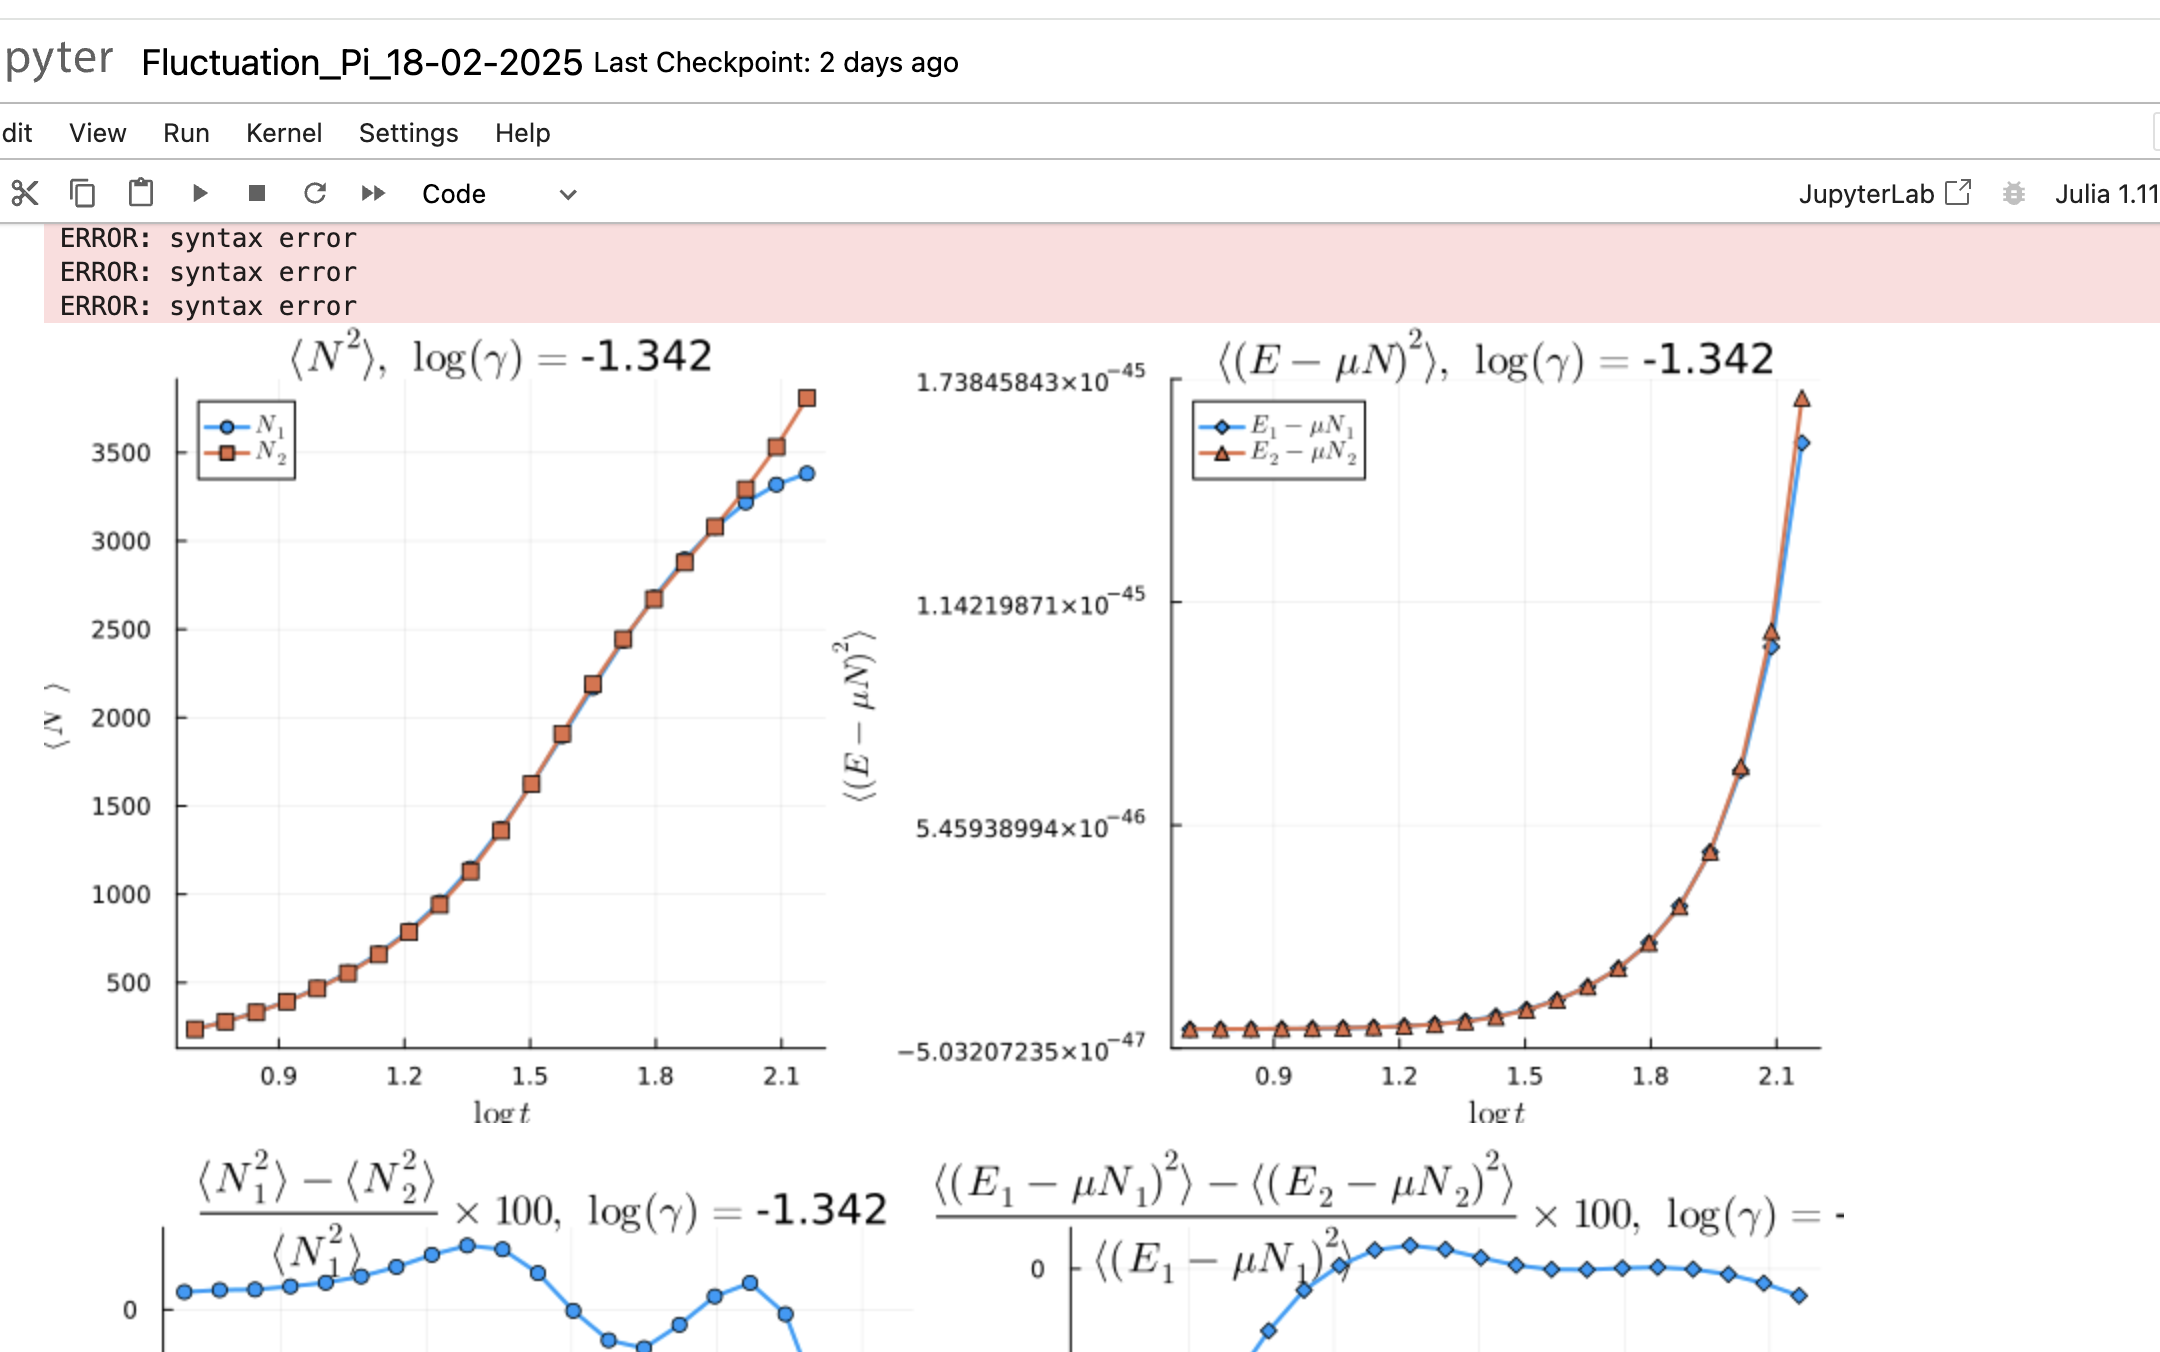
\includegraphics[width=1\textwidth]{Figures/test}

%\begin{aff}
%Donc une a l'ordre un en $\delta \theta (\operator{A}^{(0)})^{-1} %\operator{V}$ 

%\begin{eqnarray*}
%	\langle \delta \Pi ( \theta) \delta \Pi ( \theta') \rangle & = &  ( (\Pi^c_s - \Pi^c)\Pi^c/\Pi^c_s ) ( \theta ) \delta_{\theta, \theta'}/\delta \theta + \mathscr{F}(\theta , \theta' ) ,	
%\end{eqnarray*}

%avec 

%\begin{eqnarray*}
%	\mathscr{F}(\theta , \theta' ) & = & \left [ (\Pi^c_s - \Pi^c )( \theta)  +  (\Pi^c_s - \Pi^c ) ( \theta' )\right ] \frac{\Pi^c}{\Pi^c_s}(\theta)\frac{\Pi^c}{\Pi^c_s}(\theta') \frac{ \Delta( \theta'- \theta )}{ 2 \pi }\\
%	&&  - \left [ (\Pi^c_s - \Pi^c )( \theta)   (\Pi^c_s - \Pi^c ) ( \theta' )\right ] \frac{\Pi^c}{\Pi^c_s}(\theta)\frac{\Pi^c}{\Pi^c_s}(\theta')\int d\theta'' \left (   \frac{ \Pi^c/\Pi^c_s}{\Pi^c_s - \Pi^c} \right )(\theta'') \frac{\Delta(\theta''- \theta)}{2 \pi}\frac{\Delta(\theta''- \theta')}{2 \pi}  	
%\end{eqnarray*}
%\end{aff}



 









%Dans le domaine $z_1 < z_2 < \cdots < z_N$, la fonction d'onde est ({\color{blue} Gaudin 2014}, {\color{blue}Korepin et al. 1997}, {\color{blue}Lieb anz Liniger 1963}) :
%
%\begin{eqnarray}
%	\varphi_{\{\theta_a\}} ( z_1 , \cdots , z_N ) & = & \langle 0 \vert \Psi ( z_1 ) \cdots \Psi (z_N ) \vert \{ \theta_a \} \rangle \notag\\
%	& \propto & \sum_\sigma ( - 1 ) ^{ \vert \sigma \vert } \left ( \prod_{ 1 \leq a < b \leq N } ( \theta_{\sigma(b)} - \theta_{\sigma(a)} - ic ) \right ) e^{i \sum_j z_i \theta_{ \sigma(j)}}\label{eq:I-2-17},
%\end{eqnarray}

%et elle est étendue à d'autres domaines par symétrie $z_i \leftrightarrow z_j$ . Ici, la somme s'étend à toutes les permutations $\sigma$ des $N$ éléments (donc il y a $N!$ termes) et $(-1)^{|\sigma|}$ est la signature de la permutation.

%\subsection{Condition aux bords périodiques et équation de Bethe Ansatz}
%%Dans ce chapitre, nous nous intéressons aux fluctuations de la distribution de rapidité \( \delta \rho \) autour d'une distribution de référence \( \rho^c \), qui maximise la contribution à la fonction de partition des états, exprimée comme une fonctionnelle de la distribution \( \rho \) : 

La fonction de partition des états, s'exprime comme une fonctionnelle de la distribution \( \rho \) : 

\begin{eqnarray*}
	\Xi & = & \sum_\rho \exp \left( -\mathcal{A}(\rho) \right).
\end{eqnarray*}  

Dans la section {\em \bf Entropie de Yang-Yang} (\ref{??}), l'action \( \mathcal{A}(\rho) \) s'écrit sous la forme :  

\begin{eqnarray*}
	\mathcal{A}(\rho) & \doteq & - L\mathcal{S}_{YY}(\rho) + L\int f(\theta) \rho (\theta) \, d\theta,		
\end{eqnarray*}  

où \( \mathcal{S}_{YY} \) est la fonctionnelle d'entropie de Yang-Yang, définie dans (\ref{??}), et \( f \) est la fonction paramétrant les charges, introduite dans (\ref{??}).  

Dans cette même section {\em \bf Entropie de Yang-Yang} (\ref{??}), nous avons établi un lien entre \( f \) et distribution de référence \( \rho^c \), qui maximise la contribution à la fonction de partition des états .\\

On veux tester si nos experience est décrit pas un GGE. Pour cela nous nous intéressons aux fluctuations de la distribution de rapidité \( \delta \rho \) autour \( \rho^c \).

%Nous poursuivons à présent avec cette définition de l'action de classe $\mathcal{C}^2$ et admetant une distribution critique $\rho^c$ tel que sa différentielle en ce point critique soit nulle $d\mathcal{A}_{\rho^c} = 0 $ (\ref{??}) de sorte que d'aprés la formule de Taylor-Youg %afin de déterminer les fluctuations autour de \( \Pi^c \). Pour cela, nous réécrivons l'action sous la forme :  

Nous poursuivons à présent avec cette définition de l'action de classe $\mathcal{C}^2$ et admetant une distribution critique $\rho^c$ tel que sa différentielle en ce point critique soit nulle $d\mathcal{A}_{\rho^c} = 0 $ (\ref{??}) de sorte que d'aprés la formule de Taylor-Youg %afin de déterminer les fluctuations autour de \( \Pi^c \). Pour cela, nous réécrivons l'action sous la forme :  

\begin{eqnarray*}  
	\mathcal{A}(\rho^c + \delta \rho) & \underset{ \delta \rho \to 0 }{=} & \mathcal{A}(\rho^c)  + \frac{1}{2} \left. \frac{\delta^2 \mathcal{A}}{\delta \rho^2} \right|_{\rho^c} (\delta \rho) + \mathcal{O}((\delta \rho)^3),  
\end{eqnarray*}  

une expression quadratique pour l'action à l'ordre dominant en \( \delta \Pi \) avec $\left. \frac{\delta^2 \mathcal{A}}{\delta \rho^2} \right|_{\rho^c}$ la forme quadratique définie positive (Fig (\ref{fig.fluctu.A})).

\begin{figure}[H]
	\centering 
	\begin{tikzpicture}
		\begin{scope}[shift={(0,0)}]
			\begin{scope}[transform canvas={scale=0.6}]
				% Définition des couleurs avec les codes HTML
\definecolor{colorOne}{HTML}{443E46}
\definecolor{colorTwo}{HTML}{F6DEB8}
\definecolor{colorThree}{HTML}{908CA4}
\definecolor{colorFour}{HTML}{57659E}
\definecolor{colorFive}{HTML}{C57284}
\definecolor{colorSix}{HTML}{FF5B69}

% Raccourcis pour les couleurs
\def\colorOne{colorOne}
\def\colorTwo{colorTwo}
\def\colorThree{colorThree}
\def\colorFour{colorFour}
\def\colorFive{colorFive}
\def\colorSix{colorSix}

\def\colorslide{blue!50!black}



\begin{scope}
	% Tracer une courbe lisse entre des points
	\draw[shift={(0,0)} ,\colorOne]
		(-1 , 0 ) edge [thick,line width=0.8ex , ->,>=triangle 45  , \colorOne] node [pos = 1 , below ]{\huge$\rho$}( 5  , 0 )
	;
	\draw[shift={(0,0)}, color=\colorOne]
		(0, -1.0 ) edge [thick,line width=0.8ex , ->,>=triangle 45  ]node [pos=0.9,left=0.2cm ]{\huge$\mathcal{A}(\rho)$}( 0  , 5 )
	;
	\draw[]
		(2.5, 0.12 ) edge [thick,line width=0.8ex ,\colorThree ]node [pos=1,below  ]{\huge$\rho^c$} (2.5, -0.12 )	
	;
	
	\draw[]
		(2.5, -0.12 ) edge [thick,line width=0.4ex , dashed, \colorThree ] (2.5, 5.5 )
		(1.5, 1 ) edge [thick,line width=0.4ex , <->,>=triangle 45  , \colorThree ] (3.5, 1 )
		(-0.3,1) edge [thick,line width=0.4ex  , \colorThree ] node [pos=0,left ]{\huge$\mathcal{A}(\rho^c)$} (0.3, 1 )	
	;
    \draw[thick, line width=0.8ex , \colorFour] plot[smooth, tension=0.7] coordinates {
        (1, 5) (1.6 , 3 ) (2.5, 1) (3.5 , 3 )  (4, 5)
    };		
	
\end{scope}

	
			
			\end{scope}
			
			\draw[color = red , scale = 0.5 , draw = none  ] (-2 , -1) rectangle (5, 6) ; 	
		\end{scope}
		
		\begin{scope}[shift={(19,-1)}]
			\begin{scope}[transform canvas={scale=0.6}]
				% Définition des couleurs avec les codes HTML
\definecolor{colorOne}{HTML}{443E46}
\definecolor{colorTwo}{HTML}{F6DEB8}
\definecolor{colorThree}{HTML}{908CA4}
\definecolor{colorFour}{HTML}{57659E}
\definecolor{colorFive}{HTML}{C57284}
\definecolor{colorSix}{HTML}{FF5B69}

% Raccourcis pour les couleurs
\def\colorOne{colorOne}
\def\colorTwo{colorTwo}
\def\colorThree{colorThree}
\def\colorFour{colorFour}
\def\colorFive{colorFive}
\def\colorSix{colorSix}

\def\colorslide{blue!50!black}

\def\Occupation{
	\def\traitx{0.3}
	\def\traity{0.5}
	\draw[shift={(0,0)}]
		(-13.5 , 0 ) edge [thick,line width=0.8ex ]( -3.2  , 0 )
		( -3.2 - \traitx  , 0 - \traity ) edge [thick,line width=0.8ex ]( -3.2 + \traitx  , 0 + \traity  )
		( -2.8 - \traitx  , 0 - \traity ) edge [thick,line width=0.8ex ]( -2.8 + \traitx  , 0 + \traity  )
		(-2.8 , 0 ) edge [thick,line width=0.8ex ](2.8  , 0 )
		( 2.8 - \traitx  , 0 - \traity ) edge [thick,line width=0.8ex ]( 2.8 + \traitx  , 0 + \traity  )
		( 3.2 - \traitx  , 0 - \traity ) edge [thick,line width=0.8ex ]( 3.2 + \traitx  , 0 + \traity  )
		(3.2, 0 ) edge [thick,line width=0.8ex,->,>=triangle 45 , color = black ]node [pos=1.01,below  ]{\huge$\theta$}	( 13  , 0 )
	;
	\draw[shift={(0,0)}, color=\colorOne]
		(-10.5 , -1.5 ) edge [thick,line width=0.8ex , ->,>=triangle 45  ]( -10.5  , 4.5 )
	;
		
	\foreach \r in {1 , ... , 3 } {
%		\draw[
%		decoration={
%		markings,
%    	mark connection node=my node,
%    	mark=at position 0 with{\node [blue,transform shape] (my node) {\large \r};}},
%		color=gray, thick, 
%		line width=0.5ex] decorate { 
%            (-11.0, \r) -- (-10.1, \r )}
%        ;
        \draw[
			color=\colorOne,
			] 
            (-11.0, \r) edge[color=\colorThree , thick,line width=0.5ex] node [pos=-0.5 ]{\large\color{\colorFour} $\frac{\r}{\delta \theta}$ } (-10.3, \r )
        	;
	
	}
	

	
	% Graduation abcsisse 
	% Définitions des listes
% Definitions of the lists
\def\listetuple{-9/\theta_{1}, -8/\theta_{2} , -5/\theta_{3} , -2/\theta_{a-1} , 0/\theta_{a} , 1/\theta_{a+1} , 2/\theta_{a+2} ,  5/\theta_{N-4} , 7/\theta_{N-3},8/\theta_{N-1},9/\theta_{N} }
\def\listetrais{-12 , -11, -10, -9 , -8 , -7 ,  -6 , -5, -4.5,-4, -2 , -1, 0 , 0.5, 1, 2, 4 , 5 ,  6 , 7 , 8 ,8.5, 9 ,  10 , 11, 12 }

% Loop over listetrais
\foreach \r in \listetrais {
    % Initialize found variable to zero
    % Initialize found variable to zero
    %\pgfmathsetmacro\found{0}
    \global\def\found{0}
    \xdef\nomtheta{}
    
    % Check if \r is in listetuple
    \foreach \x/\y in \listetuple { 
        \ifdim \r pt=\x pt % If \r matches any \x in listetuple
            \global\def\found{1} ;
            \xdef\nomtheta{\y} % Set \nomtheta to the corresponding \y
            %\pgfmathsetmacro\found{1} % Set found to 1            
            %\global\pgfmathsetmacro\found{1}
        \fi
    }
    
    %\node [circle, draw, red] (A) at (\r, 2) {\found , $\nomtheta$};
    
    % Draw the line and display \nomtheta if found
    \ifnum\found=1
        \draw[color=\colorOne, thick, line width=0.5ex] 
            (\r, -0.3) -- (\r, 0.3) node[red , pos=-0.5] {\large $\nomtheta$};
         \filldraw[line width=0.5ex, color=\colorSix, outer color=\colorSix, inner color=\colorSix] 
            (\r, 0) circle (4pt);
    \else 
        % Draw without \nomtheta and add a blue circle if not found
        \draw[color=\colorOne, thick, line width=0.5ex] 
            (\r, -0.3) -- (\r, 0.3);
        \filldraw[line width=0.5ex, color=\colorSix, outer color=\colorTwo, inner color=\colorTwo] 
            (\r, 0) circle (4pt); 
    \fi
}

\def\listetrais{-9.5/\theta_{i-1}/2/3, -6.5/\theta_{i}/1/4  ,   -1.5/\theta_{j}/2/4 , 1.5/\theta_{j+1}/-1/3 , 3.5/\theta_{\ell-1}/1/3 , 6.5/\theta_{\ell}/3/4 , 9.5/\theta(\theta_{\ell+1})/-1/3 };



\foreach \r/\nomx/\y/\ys in \listetrais {
	\draw[
		decoration={
		markings,
    	mark connection node=my node,
    	mark=at position .5 with{\node [blue,transform shape] (my node) {\large \color{\colorFour} $\nomx$};}},
		color=\colorThree , thick, 
		line width=0.5ex] decorate { 
            (\r, 0.12) -- (\r, -1.2)}
        ;
     
     \ifdim \y pt > -1 pt 
     	\draw[
			decoration={
			markings,
    		mark connection node=my node,
    		mark=at position .5 with{\node [blue,transform shape] (my node) {\large \color{\colorFour} $\Pi(\nomx) $};}},
			color=\colorThree, thick, 
			line width=0.5ex] decorate { 
            (\r, \y) -- (\r +3, \y)}
        ;
        \draw[
			decoration={
			markings,
    		mark connection node=my node,
    		mark=at position .5 with{\node [blue,transform shape] (my node) {\large \color{\colorFive} $\Pi_s(\nomx) $};}},
			color=\colorFive, thick, 
			line width=0.5ex] decorate { 
            (\r, \ys) -- (\r +3, \ys)}
        ;
     \fi 
     \ifdim \r pt= -1.5 pt
     	\draw[
     		decoration={
			markings,
    		mark connection node=my node,
    		mark=at position .5 with{\node [blue,transform shape] (my node) {\large \color{\colorFour}  $\delta \theta $};},
    		%mark=at position 0.1  with {\arrow[blue, line width=0.5ex]{<}},
    		%mark=at position 1  with {\arrow[blue, line width=0.5ex]{>}}
    		},
        	color=\colorThree,
        	thick,
        	line width=0.5ex,
        	%arrows={Computer Modern Rightarrow[line cap=round]-Computer Modern Rightarrow[line cap=round]}
   			](\r, -1.2) edge[arrows={Computer Modern Rightarrow[line cap=round]-}] (\r + 0.4, -1.2)decorate {
    		(\r, -1.2) -- (\r + 3, -1.2)}(\r + 2, -1.2) edge[arrows={-Computer Modern Rightarrow[line cap=round]}] (\r + 3, -1.2)
    		;
    \fi
			
	
}


			
}


\begin{scope}
	%\draw[help lines , width=1.5ex] (-8,-3) grid (8,3);\draw[help lines ,width=0.5ex , opacity = 0.5] (-3,-3) grid[step=0.1] (3,3));
	
	%\draw[help lines] 
	%	(-3,-3) edge[width=1.5ex] grid (3,3)	
	%	(-3,-3) edge[width=0.5ex , opacity = 0.5] grid (3,3)	
	%;
	\begin{scope}[shift={(0,1)},rotate=0,opacity=1,color=black]
		\Occupation	
		
		%\node[anchor=east, font=\bfseries] at (-11, 0) {\color{red}\large (T = 0 )} ;	
	\end{scope}
	
	
	
	
	\begin{scope}[shift={(-10.5,7)},rotate=0,opacity=1,color=black]
	
	\begin{scope}[shift={(-0,0)},rotate=0,opacity=1,color=black]
	
		\draw[shift={(0,0)} ,line width=1ex,rounded corners = 1ex,color=\colorOne , opacity =1 ,fill=\colorOne!00 , pattern={north east lines} , pattern color=\colorOne!00 ]
			(0 , -1 ) rectangle (5,1)
		;
		

		\begin{scope}[shift={(0.5,0.5)}]
			\draw[color=\colorOne, thick, line width=0.5ex] 
            (0, -0.3) -- (0, 0.3) ;
            \filldraw[line width=0.5ex, color=\colorSix, outer color=\colorSix, inner color=\colorSix] 
            (0, 0) circle (4pt);
            
            \node[anchor=west, font=\bfseries] at (0.2, 0) {\color{\colorSix}\large : quasi-particule};
		\end{scope}
		
		\begin{scope}[shift={(0.5,-0.5)}]
			\draw[color=\colorOne, thick, line width=0.5ex] 
            (0, -0.3) -- (0, 0.3) ;
            \filldraw[line width=0.5ex, color=\colorSix, outer color=\colorTwo, inner color=\colorTwo] 
            (0, 0) circle (4pt);
            
            \node[anchor=west, font=\bfseries] at (0.2, 0) {\color{\colorSix}\large : hole};
		\end{scope}

	\end{scope}
	
	\begin{scope}[shift={(6,0)},rotate=0,opacity=1,color=black]	
		
		\draw[shift={(0,0)} ,line width=1ex,rounded corners = 1ex,color=\colorOne , opacity =1 ,fill=\colorOne!00 , pattern={north east lines} , pattern color=\colorOne!00 ]
			(0 , -1 ) rectangle (7.5,1)
		;
		
		\node[anchor=west] at (0.5, 0.5) {\color{\colorFour}\large $\Pi$ };\node[anchor=west, font=\bfseries] at (1, 0.5) {\color{\colorFour}\large : quasi-particule distribution};
		
		\node[anchor=west] at (0.5, -0.5) {\color{\colorFour}\large $\Pi_h$ };\node[anchor=west, font=\bfseries] at (1, -0.5) {\color{\colorFour}\large  : hole distribution};
		
	\end{scope}
	
	\begin{scope}[shift={(14.5,0)},rotate=0,opacity=1,color=black]	
		
		\draw[shift={(0,0)} ,line width=1ex,rounded corners = 1ex,color=\colorOne , opacity =1 ,fill=\colorOne!00 , pattern={north east lines} , pattern color=\colorOne!00 ]
			(0 , -0.5 ) rectangle (7.0,0.5)
		;
		
		\node[anchor=west] at (0.2, 0) {\color{\colorFour}\large ${\color{\colorFive}\Pi_s} = \Pi + \Pi_h $ } node[anchor=west , font=\bfseries] at (3.1 , 0 )  {\color{\colorFour}\large {\color{\colorFive} : density of states}};
		
	\end{scope}
	
	
	\end{scope}


		
	
\end{scope}

	
			
			\end{scope}
			\begin{scope}[scale=1]
				\draw[color = red , scale = 1 , draw = none  ] (-1 , -1) rectangle (5, 5) ; 
			\end{scope}	
		\end{scope}

		
				
			
	\end{tikzpicture}	
	\captionsetup{skip=10pt} % Ajoute de l’espace après la légende
	\label{fig.fluctu.A}
\end{figure}


On discrétise l'axe des rapidités en  petite cellule de rapidité $[\theta, \theta+\delta\theta]$, qui contient $L\rho(\theta) \delta \theta$ rapidités. 
	



Avec ces petites tranches, la forme quadratique s’écrit :

\begin{eqnarray*}
    \left. \frac{\delta^2 \mathcal{A}}{{\delta \rho}^2} \right|_{\rho^c}(\delta \rho ) &=&  \sum_{a,b \mid \text{tranche}}  
    \delta \rho(\theta_a)  \frac{\partial^2 \mathcal{A}}{\partial \delta \rho(\theta_a) \partial \delta \rho(\theta_b) } (\rho^c)  \delta \rho(\theta_b).
\end{eqnarray*}
Les fluctuations s’écrivent donc :

\begin{eqnarray*}
    \langle \delta \rho ( \theta) \delta \rho ( \theta') \rangle &=&  
    \frac{ \int d\delta \rho \, \delta \rho(\theta) \delta \rho ( \theta') 
    \exp \left( - \frac{1}{2} \sum_{a,b \mid \text{tranche}}  
    \delta \rho(\theta_a) \frac{\partial^2 \mathcal{A}}{\partial \delta \rho(\theta_a) \partial \delta \rho(\theta_b) } (\rho^c)  \delta \rho(\theta_b) \right) }
    { \int d\delta \Pi  
    \exp \left( - \frac{1}{2} \sum_{a,b \mid \text{tranche}}  
    \delta \rho(\theta_a) \frac{\partial^2 \mathcal{A}}{\partial \delta \rho(\theta_a) \partial \delta \rho(\theta_b) } (\rho^c)  \delta \rho(\theta_b) \right) } \\
    &=& \left( \mathbf{A}^{-1} \right)_{\theta , \theta'}
\end{eqnarray*}


\begin{aff}

\begin{eqnarray*}
	\langle \delta \rho ( \theta) \delta \rho ( \theta') \rangle &=& 	\left( \mathbf{A}^{-1} \right)_{\theta , \theta'}
\end{eqnarray*}

	
avec la  {\em matrice hessienne} $\mathbf{A}_{\theta , \theta'} \equiv \frac{\partial^2 \mathcal{A}}{\partial \delta \rho(\theta) \partial \delta \rho(\theta') }(\rho^c)$, au point critique/ qui maximise la probabilité  $\rho^c=\rho^c_s \nu^c $, s'écrit

\begin{eqnarray*}
	\operator{A} & = & \operator{A}^{(0)} + \delta \theta \operator{V}
\end{eqnarray*}

avec 

\begin{eqnarray*}
	A^{(0)}_{\theta , \theta'}  & = &  L\delta \theta \left ( \frac{ 1}{\rho^c_s ( 1  - \nu^c ) \nu^c } \right )(\theta)    \delta({\theta - \theta '})	,\\
	V_{\theta , \theta'}  &= & L \delta \theta \left \{ - \left [ \left ( \frac{1}{\rho^c_s( 1 - \nu^c) } \right ) ( \theta)  +  \left ( \frac{1}{\rho^c_s( 1 - \nu^c) } \right ) ( \theta' )\right ] \frac{ \Delta( \theta'- \theta )}{ 2 \pi } + \int d\theta''  \left ( \frac{\nu^c}{\rho^c_s( 1 - \nu^c) } \right )(\theta'') \frac{\Delta(\theta''- \theta)}{2 \pi}\frac{\Delta(\theta''- \theta')}{2 \pi}   \right \} 	
\end{eqnarray*}

\end{aff}

\subsection{Testes}

\begin{eqnarray*}
	\Delta_{\operator{\mathcal{N}}}^2  & = &  \frac{1}{\beta} \left . \frac{\partial \langle \operator{\mathcal{N}} \rangle}{\partial \mu} \right )_T \\
	\Delta_{\operator{\mathcal{E}}-\mu \operator{\mathcal{N}}}^2  & = &  - \left . \frac{\partial \langle \operator{\mathcal{E}}-\mu \operator{\mathcal{N}} \rangle}{\partial \beta} \right )_\mu 
\end{eqnarray*}

et 

\begin{eqnarray*}
	\Delta_{\operator{\mathcal{N}}}^2  &= & L^2 \int d\theta_a \int d \theta_b \, \langle \delta \rho(\theta_a) \delta \rho(\theta_b) \rangle \\
	\Delta_{\operator{\mathcal{E}}-\mu \operator{\mathcal{N}}}^2  & = & L^2 \int d\theta_a \int d \theta_b \, \left ( - \mu + \frac{1}2 m \theta_a^2  \right  )\left ( - \mu + \frac{1}2 m \theta_b^2  \right  )  \langle \delta \rho(\theta_a) \delta \rho(\theta_b) \rangle
\end{eqnarray*}

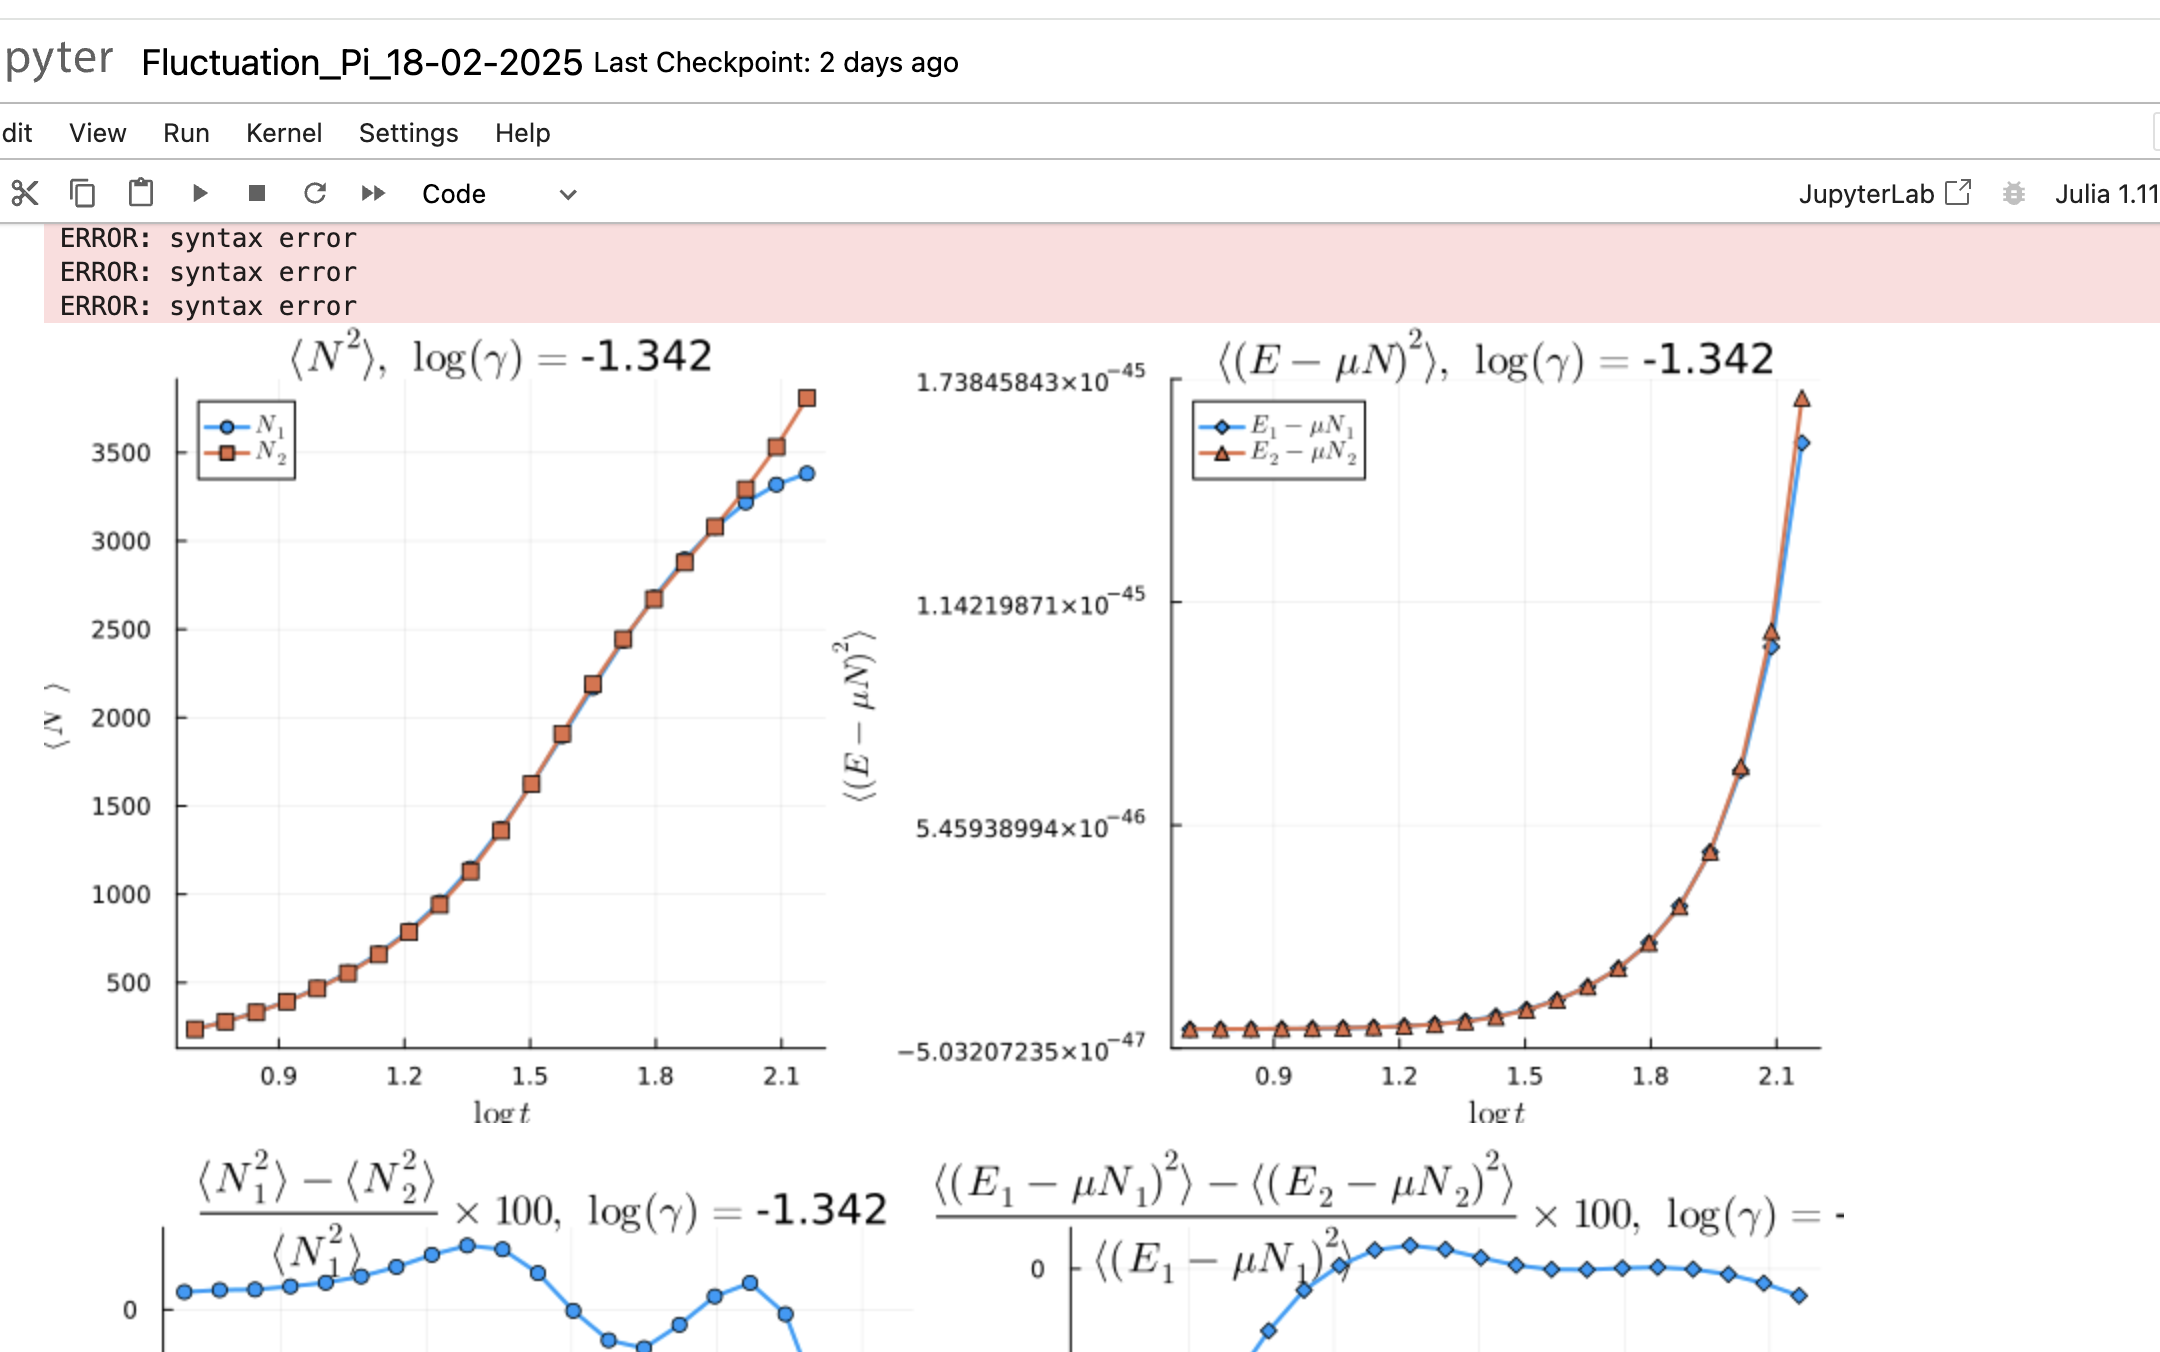
\includegraphics[width=1\textwidth]{Figures/test}

%\begin{aff}
%Donc une a l'ordre un en $\delta \theta (\operator{A}^{(0)})^{-1} %\operator{V}$ 

%\begin{eqnarray*}
%	\langle \delta \Pi ( \theta) \delta \Pi ( \theta') \rangle & = &  ( (\Pi^c_s - \Pi^c)\Pi^c/\Pi^c_s ) ( \theta ) \delta_{\theta, \theta'}/\delta \theta + \mathscr{F}(\theta , \theta' ) ,	
%\end{eqnarray*}

%avec 

%\begin{eqnarray*}
%	\mathscr{F}(\theta , \theta' ) & = & \left [ (\Pi^c_s - \Pi^c )( \theta)  +  (\Pi^c_s - \Pi^c ) ( \theta' )\right ] \frac{\Pi^c}{\Pi^c_s}(\theta)\frac{\Pi^c}{\Pi^c_s}(\theta') \frac{ \Delta( \theta'- \theta )}{ 2 \pi }\\
%	&&  - \left [ (\Pi^c_s - \Pi^c )( \theta)   (\Pi^c_s - \Pi^c ) ( \theta' )\right ] \frac{\Pi^c}{\Pi^c_s}(\theta)\frac{\Pi^c}{\Pi^c_s}(\theta')\int d\theta'' \left (   \frac{ \Pi^c/\Pi^c_s}{\Pi^c_s - \Pi^c} \right )(\theta'') \frac{\Delta(\theta''- \theta)}{2 \pi}\frac{\Delta(\theta''- \theta')}{2 \pi}  	
%\end{eqnarray*}
%\end{aff}



 










\subsection{Fonction d’onde dans le secteur ordonné et représentation de Gaudin}

Dans le domaine $z_1 < z_2 < \cdots < z_N$, la fonction d’onde pour un état de Bethe à $N$ particules s’écrit ({\color{blue}Gaudin 2014}, {\color{blue}Korepin et al. 1997}, {\color{black}Lieb et Liniger 1963}) :
\begin{eqnarray}
	\varphi_{\{\theta_a\}} ( z_1 , \cdots , z_N ) & = &  \frac{1}{\sqrt{N!}}\langle \emptyset \vert \operator{\Psi} ( z_1 ) \cdots \operator{\Psi} (z_N ) \vert \{ \theta_a \} \rangle \notag\\
	& \propto & \sum_\sigma (-1)^{|\sigma|} \left( \prod_{1 \leq a < b \leq N} (\theta_{\sigma(b)} - \theta_{\sigma(a)} - i g) \right) e^{i \sum_{j=1}^{N} z_j \theta_{\sigma(j)}},\label{eq:I-2-17}
\end{eqnarray}
où la somme s'étend sur toutes les permutations $\sigma$ de $\{1,\dots,N\}$. Le facteur $(-1)^{|\sigma|}$ est la signature de la permutation, et les amplitudes dépendent des différences de quasi-moments $\theta_j$ ainsi que du couplage $c$.
Cette fonction d’onde est ensuite étendue par symétrie aux autres domaines du type $z_{\pi(1)} < z_{\pi(2)} < \cdots < z_{\pi(N)}$ via des propriétés d’échange symétriques.

\vspace{1em}

\subsection{Conditions aux bords périodiques}

Les équations précédentes ont été établies pour un système défini sur la droite réelle. Cependant, dans une perspective thermodynamique, il est essentiel de considérer une densité finie $ N/L$. Cela peut être obtenu en compactifiant l’espace sur un cercle de longueur $L$, i.e. en imposant les {\em conditions aux bords périodiques}.

Concrètement, cela consiste à identifier $x = 0$ et $x = L$ et à exiger que la fonction d’onde soit périodique lorsqu’une particule fait le tour du système :
\begin{equation}\label{eq:periodic}
\varphi_{\{\theta_a\}}(x_1, \dots, x_{N-1}, L) = \varphi_{\{\theta_a\}}(0, x_1, \dots, x_{N-1}).
\end{equation}
Cette condition doit être satisfaite pour chaque particule. Or, déplacer la $j$-ième particule de $x_j$ à $x_j + L$ revient à la faire passer devant toutes les autres : cela introduit un facteur de diffusion à chaque croisement.

%\vspace{1em}

\subsection{Équations de Bethe exponentielles}

En imposant les conditions de périodicité sur la fonction d’onde de type Bethe~\eqref{eq:I-2-17}, on obtient que chaque moment $\theta_a$ doit satisfaire l’équation :
\begin{equation}
	e^{i \theta_a L} \prod_{b \ne a} S(\theta_a - \theta_b) = (-1)^{N-1}, \quad a = 1, \dots, N,
	\label{eq:bethe_exp}
\end{equation}
où la matrice diffusion $S(\theta) = \frac{\theta - i g}{-\theta - i g} = e^{i \Phi(\theta)}$ est l’amplitude de diffusion à deux corps, et $\Phi(\theta) = 2 \arctan\left( \frac{\theta}{c} \right)$ est la phase associée~\eqref{chap:1:eq:Phi}. Le signe $(-1)^{N-1}$ vient du fait que chaque permutation change la signature du déterminant dans la représentation de Gaudin.
%\vspace{1em}

\subsection{Équations de Bethe logarithmiques}

En prenant le logarithme du membre gauche et du membre droit de l’équation~\eqref{eq:bethe_exp}, on obtient :
\begin{equation}\label{chap:1:eq:EBA}
	L \theta_a + \sum_{b=1}^N \Phi(\theta_a - \theta_b) = 2\pi I_a, \qquad a = 1, \dots, N,
\end{equation}
où les $I_a \in \mathbb{Z}$ (ou $\mathbb{Z} + \tfrac{1}{2}$) sont des nombres quantiques entiers (ou demis entiers) . Dans la configuration d’état fondamental (ou de type “mer de Fermi”), ces nombres sont pris de manière symétrique autour de zéro :
\[
I_a = a - \frac{N+1}{2}, \quad \text{pour } a \in \llbracket 1 , N \rrbracket.
\]
Ce choix garantit une distribution uniforme des $\theta_a$ à l’état fondamental.
%\vspace{1em}

\subsection{Interprétation physique}

Les équations de Bethe~\eqref{chap:1:eq:EBA} représentent une {\em quantification des pseudo‑impulsions $\theta_a$} des particules en interaction, résultant d’un {\em interféromètre multi‑corps sur le cercle} : chaque particule accumule une phase $e^{i \theta_a L}$ due au mouvement libre, ainsi que des phases de diffusion lorsqu’elle croise les autres.

Ce système d'équations détermine les états propres du système de Lieb–Liniger en volume fini, et joue un rôle fondamental dans la description exacte de ses propriétés thermodynamiques et dynamiques.


\subsection{Thermodynamique du gaz de Lieb–Liniger à température nulle}

Dans la limite thermodynamique, le nombre de particules \( N \) et la longueur \( L \) du système tendent vers l'infini de telle sorte que leur rapport reste fini :
\begin{eqnarray*}
	\lim_{N,\, L \to \infty} \frac{N}{L} = D < \infty,
\end{eqnarray*}
où \( D \) désigne la densité linéique de particules.

Considérons désormais le système à température nulle. L’état fondamental dans le secteur à nombre de particules fixé correspond à la configuration d’énergie minimale parmi les solutions des équations de Bethe \eqref{chap:1:eq:EBA}.

Dans la limite thermodynamique, les valeurs de \( \theta_a \) deviennent quasi-continues, avec un espacement \( \theta_{a+1} - \theta_a = \mathcal{O}(1/L) \), et se condensent dans un intervalle symétrique autour de zéro :
\[
\theta_a \in [-K, K],
\]
où \( K \) est le paramètre de Fermi (ou rapidité maximale), défini par \( K = \theta_N \). En supposant l'ordre \( I_a \geq I_b \Rightarrow \theta_a \geq \theta_b \), cet intervalle constitue ce qu'on appelle la {\em mer de Dirac} (ou sphère de Fermi en dimension un).

Nous introduisons la densité d’états \( \rho_s(\theta) \), définie par
\begin{eqnarray*}
	2\pi \rho_s(\theta_a) &=& \frac{2\pi}{L} \lim_{\text{therm}} \frac{|I_{a+1} - I_a|}{|\theta_{a+1} - \theta_a|} = \frac{2\pi}{L} \frac{\partial I}{\partial \theta}(\theta_a),
\end{eqnarray*}
où \( I(\theta_a) = I_a \). L’application des équations de Bethe sous forme logarithmique conduit alors à
\begin{eqnarray*}
	2\pi \rho_s(\theta_a) = 1 + \frac{1}{L} \sum_{b = 1}^N \Delta(\theta_a - \theta_b),
\end{eqnarray*}
ce qui relie \( \rho_s \) à la fonction d’interaction \( \Delta \) entre les rapidités.

Intéressons-nous maintenant à la {\em densité de particules dans l’espace des moments}, notée \( \rho(\theta) \), définie par
\begin{eqnarray*}
	\rho(\theta_a) = \lim_{L \to \infty} \frac{1}{L} \cdot \frac{1}{\theta_{a+1} - \theta_a} > 0.
\end{eqnarray*}
Dans l’état fondamental, toutes les positions disponibles dans l’intervalle \( [-K, K] \) sont occupées. On a donc :
\begin{eqnarray}\label{chap.1.rho.2}
	\rho(\theta) = \rho_s(\theta).
\end{eqnarray}

La quantité \( L \rho(\theta) d\theta \) représente le nombre de rapidités dans la cellule infinitésimale \( [\theta, \theta + d\theta] \), tandis que
\(
	N = L \int_{-K}^{K} \rho(\theta)\, d\theta
\)
donne le nombre total de particules dans le système. Le passage de la somme discrète à l'intégrale dans le second membre de l'équation de Bethe permet d’écrire :
\begin{eqnarray*}
	\frac{1}{L} \sum_{b = 1}^N \Delta(\theta_a - \theta_b) \longrightarrow \int_{-K}^{K} \Delta(\theta_a - \theta)\, \rho(\theta)\, d\theta.
\end{eqnarray*}
Ainsi, l'équation pour la densité d'états devient :
\begin{eqnarray}\label{chap.1.rho.s.2}
	2\pi \rho_s(\theta) = 1 + \int_{-K}^{K} \Delta(\theta - \theta')\, \rho(\theta')\, d\theta',
\end{eqnarray}
et, comme \( \rho = \rho_s \), on obtient l’équation linéaire intégrale satisfaite par la densité de rapidités :
\begin{eqnarray}\label{chap.1.rho.3}
	\rho(\theta) - \int_{-K}^{K} \frac{\Delta(\theta - \theta')}{2\pi} \rho(\theta')\, d\theta' = \frac{1}{2\pi}.
\end{eqnarray}


%%Dans ce chapitre, nous nous intéressons aux fluctuations de la distribution de rapidité \( \delta \rho \) autour d'une distribution de référence \( \rho^c \), qui maximise la contribution à la fonction de partition des états, exprimée comme une fonctionnelle de la distribution \( \rho \) : 

La fonction de partition des états, s'exprime comme une fonctionnelle de la distribution \( \rho \) : 

\begin{eqnarray*}
	\Xi & = & \sum_\rho \exp \left( -\mathcal{A}(\rho) \right).
\end{eqnarray*}  

Dans la section {\em \bf Entropie de Yang-Yang} (\ref{??}), l'action \( \mathcal{A}(\rho) \) s'écrit sous la forme :  

\begin{eqnarray*}
	\mathcal{A}(\rho) & \doteq & - L\mathcal{S}_{YY}(\rho) + L\int f(\theta) \rho (\theta) \, d\theta,		
\end{eqnarray*}  

où \( \mathcal{S}_{YY} \) est la fonctionnelle d'entropie de Yang-Yang, définie dans (\ref{??}), et \( f \) est la fonction paramétrant les charges, introduite dans (\ref{??}).  

Dans cette même section {\em \bf Entropie de Yang-Yang} (\ref{??}), nous avons établi un lien entre \( f \) et distribution de référence \( \rho^c \), qui maximise la contribution à la fonction de partition des états .\\

On veux tester si nos experience est décrit pas un GGE. Pour cela nous nous intéressons aux fluctuations de la distribution de rapidité \( \delta \rho \) autour \( \rho^c \).

%Nous poursuivons à présent avec cette définition de l'action de classe $\mathcal{C}^2$ et admetant une distribution critique $\rho^c$ tel que sa différentielle en ce point critique soit nulle $d\mathcal{A}_{\rho^c} = 0 $ (\ref{??}) de sorte que d'aprés la formule de Taylor-Youg %afin de déterminer les fluctuations autour de \( \Pi^c \). Pour cela, nous réécrivons l'action sous la forme :  

Nous poursuivons à présent avec cette définition de l'action de classe $\mathcal{C}^2$ et admetant une distribution critique $\rho^c$ tel que sa différentielle en ce point critique soit nulle $d\mathcal{A}_{\rho^c} = 0 $ (\ref{??}) de sorte que d'aprés la formule de Taylor-Youg %afin de déterminer les fluctuations autour de \( \Pi^c \). Pour cela, nous réécrivons l'action sous la forme :  

\begin{eqnarray*}  
	\mathcal{A}(\rho^c + \delta \rho) & \underset{ \delta \rho \to 0 }{=} & \mathcal{A}(\rho^c)  + \frac{1}{2} \left. \frac{\delta^2 \mathcal{A}}{\delta \rho^2} \right|_{\rho^c} (\delta \rho) + \mathcal{O}((\delta \rho)^3),  
\end{eqnarray*}  

une expression quadratique pour l'action à l'ordre dominant en \( \delta \Pi \) avec $\left. \frac{\delta^2 \mathcal{A}}{\delta \rho^2} \right|_{\rho^c}$ la forme quadratique définie positive (Fig (\ref{fig.fluctu.A})).

\begin{figure}[H]
	\centering 
	\begin{tikzpicture}
		\begin{scope}[shift={(0,0)}]
			\begin{scope}[transform canvas={scale=0.6}]
				% Définition des couleurs avec les codes HTML
\definecolor{colorOne}{HTML}{443E46}
\definecolor{colorTwo}{HTML}{F6DEB8}
\definecolor{colorThree}{HTML}{908CA4}
\definecolor{colorFour}{HTML}{57659E}
\definecolor{colorFive}{HTML}{C57284}
\definecolor{colorSix}{HTML}{FF5B69}

% Raccourcis pour les couleurs
\def\colorOne{colorOne}
\def\colorTwo{colorTwo}
\def\colorThree{colorThree}
\def\colorFour{colorFour}
\def\colorFive{colorFive}
\def\colorSix{colorSix}

\def\colorslide{blue!50!black}



\begin{scope}
	% Tracer une courbe lisse entre des points
	\draw[shift={(0,0)} ,\colorOne]
		(-1 , 0 ) edge [thick,line width=0.8ex , ->,>=triangle 45  , \colorOne] node [pos = 1 , below ]{\huge$\rho$}( 5  , 0 )
	;
	\draw[shift={(0,0)}, color=\colorOne]
		(0, -1.0 ) edge [thick,line width=0.8ex , ->,>=triangle 45  ]node [pos=0.9,left=0.2cm ]{\huge$\mathcal{A}(\rho)$}( 0  , 5 )
	;
	\draw[]
		(2.5, 0.12 ) edge [thick,line width=0.8ex ,\colorThree ]node [pos=1,below  ]{\huge$\rho^c$} (2.5, -0.12 )	
	;
	
	\draw[]
		(2.5, -0.12 ) edge [thick,line width=0.4ex , dashed, \colorThree ] (2.5, 5.5 )
		(1.5, 1 ) edge [thick,line width=0.4ex , <->,>=triangle 45  , \colorThree ] (3.5, 1 )
		(-0.3,1) edge [thick,line width=0.4ex  , \colorThree ] node [pos=0,left ]{\huge$\mathcal{A}(\rho^c)$} (0.3, 1 )	
	;
    \draw[thick, line width=0.8ex , \colorFour] plot[smooth, tension=0.7] coordinates {
        (1, 5) (1.6 , 3 ) (2.5, 1) (3.5 , 3 )  (4, 5)
    };		
	
\end{scope}

	
			
			\end{scope}
			
			\draw[color = red , scale = 0.5 , draw = none  ] (-2 , -1) rectangle (5, 6) ; 	
		\end{scope}
		
		\begin{scope}[shift={(19,-1)}]
			\begin{scope}[transform canvas={scale=0.6}]
				% Définition des couleurs avec les codes HTML
\definecolor{colorOne}{HTML}{443E46}
\definecolor{colorTwo}{HTML}{F6DEB8}
\definecolor{colorThree}{HTML}{908CA4}
\definecolor{colorFour}{HTML}{57659E}
\definecolor{colorFive}{HTML}{C57284}
\definecolor{colorSix}{HTML}{FF5B69}

% Raccourcis pour les couleurs
\def\colorOne{colorOne}
\def\colorTwo{colorTwo}
\def\colorThree{colorThree}
\def\colorFour{colorFour}
\def\colorFive{colorFive}
\def\colorSix{colorSix}

\def\colorslide{blue!50!black}

\def\Occupation{
	\def\traitx{0.3}
	\def\traity{0.5}
	\draw[shift={(0,0)}]
		(-13.5 , 0 ) edge [thick,line width=0.8ex ]( -3.2  , 0 )
		( -3.2 - \traitx  , 0 - \traity ) edge [thick,line width=0.8ex ]( -3.2 + \traitx  , 0 + \traity  )
		( -2.8 - \traitx  , 0 - \traity ) edge [thick,line width=0.8ex ]( -2.8 + \traitx  , 0 + \traity  )
		(-2.8 , 0 ) edge [thick,line width=0.8ex ](2.8  , 0 )
		( 2.8 - \traitx  , 0 - \traity ) edge [thick,line width=0.8ex ]( 2.8 + \traitx  , 0 + \traity  )
		( 3.2 - \traitx  , 0 - \traity ) edge [thick,line width=0.8ex ]( 3.2 + \traitx  , 0 + \traity  )
		(3.2, 0 ) edge [thick,line width=0.8ex,->,>=triangle 45 , color = black ]node [pos=1.01,below  ]{\huge$\theta$}	( 13  , 0 )
	;
	\draw[shift={(0,0)}, color=\colorOne]
		(-10.5 , -1.5 ) edge [thick,line width=0.8ex , ->,>=triangle 45  ]( -10.5  , 4.5 )
	;
		
	\foreach \r in {1 , ... , 3 } {
%		\draw[
%		decoration={
%		markings,
%    	mark connection node=my node,
%    	mark=at position 0 with{\node [blue,transform shape] (my node) {\large \r};}},
%		color=gray, thick, 
%		line width=0.5ex] decorate { 
%            (-11.0, \r) -- (-10.1, \r )}
%        ;
        \draw[
			color=\colorOne,
			] 
            (-11.0, \r) edge[color=\colorThree , thick,line width=0.5ex] node [pos=-0.5 ]{\large\color{\colorFour} $\frac{\r}{\delta \theta}$ } (-10.3, \r )
        	;
	
	}
	

	
	% Graduation abcsisse 
	% Définitions des listes
% Definitions of the lists
\def\listetuple{-9/\theta_{1}, -8/\theta_{2} , -5/\theta_{3} , -2/\theta_{a-1} , 0/\theta_{a} , 1/\theta_{a+1} , 2/\theta_{a+2} ,  5/\theta_{N-4} , 7/\theta_{N-3},8/\theta_{N-1},9/\theta_{N} }
\def\listetrais{-12 , -11, -10, -9 , -8 , -7 ,  -6 , -5, -4.5,-4, -2 , -1, 0 , 0.5, 1, 2, 4 , 5 ,  6 , 7 , 8 ,8.5, 9 ,  10 , 11, 12 }

% Loop over listetrais
\foreach \r in \listetrais {
    % Initialize found variable to zero
    % Initialize found variable to zero
    %\pgfmathsetmacro\found{0}
    \global\def\found{0}
    \xdef\nomtheta{}
    
    % Check if \r is in listetuple
    \foreach \x/\y in \listetuple { 
        \ifdim \r pt=\x pt % If \r matches any \x in listetuple
            \global\def\found{1} ;
            \xdef\nomtheta{\y} % Set \nomtheta to the corresponding \y
            %\pgfmathsetmacro\found{1} % Set found to 1            
            %\global\pgfmathsetmacro\found{1}
        \fi
    }
    
    %\node [circle, draw, red] (A) at (\r, 2) {\found , $\nomtheta$};
    
    % Draw the line and display \nomtheta if found
    \ifnum\found=1
        \draw[color=\colorOne, thick, line width=0.5ex] 
            (\r, -0.3) -- (\r, 0.3) node[red , pos=-0.5] {\large $\nomtheta$};
         \filldraw[line width=0.5ex, color=\colorSix, outer color=\colorSix, inner color=\colorSix] 
            (\r, 0) circle (4pt);
    \else 
        % Draw without \nomtheta and add a blue circle if not found
        \draw[color=\colorOne, thick, line width=0.5ex] 
            (\r, -0.3) -- (\r, 0.3);
        \filldraw[line width=0.5ex, color=\colorSix, outer color=\colorTwo, inner color=\colorTwo] 
            (\r, 0) circle (4pt); 
    \fi
}

\def\listetrais{-9.5/\theta_{i-1}/2/3, -6.5/\theta_{i}/1/4  ,   -1.5/\theta_{j}/2/4 , 1.5/\theta_{j+1}/-1/3 , 3.5/\theta_{\ell-1}/1/3 , 6.5/\theta_{\ell}/3/4 , 9.5/\theta(\theta_{\ell+1})/-1/3 };



\foreach \r/\nomx/\y/\ys in \listetrais {
	\draw[
		decoration={
		markings,
    	mark connection node=my node,
    	mark=at position .5 with{\node [blue,transform shape] (my node) {\large \color{\colorFour} $\nomx$};}},
		color=\colorThree , thick, 
		line width=0.5ex] decorate { 
            (\r, 0.12) -- (\r, -1.2)}
        ;
     
     \ifdim \y pt > -1 pt 
     	\draw[
			decoration={
			markings,
    		mark connection node=my node,
    		mark=at position .5 with{\node [blue,transform shape] (my node) {\large \color{\colorFour} $\Pi(\nomx) $};}},
			color=\colorThree, thick, 
			line width=0.5ex] decorate { 
            (\r, \y) -- (\r +3, \y)}
        ;
        \draw[
			decoration={
			markings,
    		mark connection node=my node,
    		mark=at position .5 with{\node [blue,transform shape] (my node) {\large \color{\colorFive} $\Pi_s(\nomx) $};}},
			color=\colorFive, thick, 
			line width=0.5ex] decorate { 
            (\r, \ys) -- (\r +3, \ys)}
        ;
     \fi 
     \ifdim \r pt= -1.5 pt
     	\draw[
     		decoration={
			markings,
    		mark connection node=my node,
    		mark=at position .5 with{\node [blue,transform shape] (my node) {\large \color{\colorFour}  $\delta \theta $};},
    		%mark=at position 0.1  with {\arrow[blue, line width=0.5ex]{<}},
    		%mark=at position 1  with {\arrow[blue, line width=0.5ex]{>}}
    		},
        	color=\colorThree,
        	thick,
        	line width=0.5ex,
        	%arrows={Computer Modern Rightarrow[line cap=round]-Computer Modern Rightarrow[line cap=round]}
   			](\r, -1.2) edge[arrows={Computer Modern Rightarrow[line cap=round]-}] (\r + 0.4, -1.2)decorate {
    		(\r, -1.2) -- (\r + 3, -1.2)}(\r + 2, -1.2) edge[arrows={-Computer Modern Rightarrow[line cap=round]}] (\r + 3, -1.2)
    		;
    \fi
			
	
}


			
}


\begin{scope}
	%\draw[help lines , width=1.5ex] (-8,-3) grid (8,3);\draw[help lines ,width=0.5ex , opacity = 0.5] (-3,-3) grid[step=0.1] (3,3));
	
	%\draw[help lines] 
	%	(-3,-3) edge[width=1.5ex] grid (3,3)	
	%	(-3,-3) edge[width=0.5ex , opacity = 0.5] grid (3,3)	
	%;
	\begin{scope}[shift={(0,1)},rotate=0,opacity=1,color=black]
		\Occupation	
		
		%\node[anchor=east, font=\bfseries] at (-11, 0) {\color{red}\large (T = 0 )} ;	
	\end{scope}
	
	
	
	
	\begin{scope}[shift={(-10.5,7)},rotate=0,opacity=1,color=black]
	
	\begin{scope}[shift={(-0,0)},rotate=0,opacity=1,color=black]
	
		\draw[shift={(0,0)} ,line width=1ex,rounded corners = 1ex,color=\colorOne , opacity =1 ,fill=\colorOne!00 , pattern={north east lines} , pattern color=\colorOne!00 ]
			(0 , -1 ) rectangle (5,1)
		;
		

		\begin{scope}[shift={(0.5,0.5)}]
			\draw[color=\colorOne, thick, line width=0.5ex] 
            (0, -0.3) -- (0, 0.3) ;
            \filldraw[line width=0.5ex, color=\colorSix, outer color=\colorSix, inner color=\colorSix] 
            (0, 0) circle (4pt);
            
            \node[anchor=west, font=\bfseries] at (0.2, 0) {\color{\colorSix}\large : quasi-particule};
		\end{scope}
		
		\begin{scope}[shift={(0.5,-0.5)}]
			\draw[color=\colorOne, thick, line width=0.5ex] 
            (0, -0.3) -- (0, 0.3) ;
            \filldraw[line width=0.5ex, color=\colorSix, outer color=\colorTwo, inner color=\colorTwo] 
            (0, 0) circle (4pt);
            
            \node[anchor=west, font=\bfseries] at (0.2, 0) {\color{\colorSix}\large : hole};
		\end{scope}

	\end{scope}
	
	\begin{scope}[shift={(6,0)},rotate=0,opacity=1,color=black]	
		
		\draw[shift={(0,0)} ,line width=1ex,rounded corners = 1ex,color=\colorOne , opacity =1 ,fill=\colorOne!00 , pattern={north east lines} , pattern color=\colorOne!00 ]
			(0 , -1 ) rectangle (7.5,1)
		;
		
		\node[anchor=west] at (0.5, 0.5) {\color{\colorFour}\large $\Pi$ };\node[anchor=west, font=\bfseries] at (1, 0.5) {\color{\colorFour}\large : quasi-particule distribution};
		
		\node[anchor=west] at (0.5, -0.5) {\color{\colorFour}\large $\Pi_h$ };\node[anchor=west, font=\bfseries] at (1, -0.5) {\color{\colorFour}\large  : hole distribution};
		
	\end{scope}
	
	\begin{scope}[shift={(14.5,0)},rotate=0,opacity=1,color=black]	
		
		\draw[shift={(0,0)} ,line width=1ex,rounded corners = 1ex,color=\colorOne , opacity =1 ,fill=\colorOne!00 , pattern={north east lines} , pattern color=\colorOne!00 ]
			(0 , -0.5 ) rectangle (7.0,0.5)
		;
		
		\node[anchor=west] at (0.2, 0) {\color{\colorFour}\large ${\color{\colorFive}\Pi_s} = \Pi + \Pi_h $ } node[anchor=west , font=\bfseries] at (3.1 , 0 )  {\color{\colorFour}\large {\color{\colorFive} : density of states}};
		
	\end{scope}
	
	
	\end{scope}


		
	
\end{scope}

	
			
			\end{scope}
			\begin{scope}[scale=1]
				\draw[color = red , scale = 1 , draw = none  ] (-1 , -1) rectangle (5, 5) ; 
			\end{scope}	
		\end{scope}

		
				
			
	\end{tikzpicture}	
	\captionsetup{skip=10pt} % Ajoute de l’espace après la légende
	\label{fig.fluctu.A}
\end{figure}


On discrétise l'axe des rapidités en  petite cellule de rapidité $[\theta, \theta+\delta\theta]$, qui contient $L\rho(\theta) \delta \theta$ rapidités. 
	



Avec ces petites tranches, la forme quadratique s’écrit :

\begin{eqnarray*}
    \left. \frac{\delta^2 \mathcal{A}}{{\delta \rho}^2} \right|_{\rho^c}(\delta \rho ) &=&  \sum_{a,b \mid \text{tranche}}  
    \delta \rho(\theta_a)  \frac{\partial^2 \mathcal{A}}{\partial \delta \rho(\theta_a) \partial \delta \rho(\theta_b) } (\rho^c)  \delta \rho(\theta_b).
\end{eqnarray*}
Les fluctuations s’écrivent donc :

\begin{eqnarray*}
    \langle \delta \rho ( \theta) \delta \rho ( \theta') \rangle &=&  
    \frac{ \int d\delta \rho \, \delta \rho(\theta) \delta \rho ( \theta') 
    \exp \left( - \frac{1}{2} \sum_{a,b \mid \text{tranche}}  
    \delta \rho(\theta_a) \frac{\partial^2 \mathcal{A}}{\partial \delta \rho(\theta_a) \partial \delta \rho(\theta_b) } (\rho^c)  \delta \rho(\theta_b) \right) }
    { \int d\delta \Pi  
    \exp \left( - \frac{1}{2} \sum_{a,b \mid \text{tranche}}  
    \delta \rho(\theta_a) \frac{\partial^2 \mathcal{A}}{\partial \delta \rho(\theta_a) \partial \delta \rho(\theta_b) } (\rho^c)  \delta \rho(\theta_b) \right) } \\
    &=& \left( \mathbf{A}^{-1} \right)_{\theta , \theta'}
\end{eqnarray*}


\begin{aff}

\begin{eqnarray*}
	\langle \delta \rho ( \theta) \delta \rho ( \theta') \rangle &=& 	\left( \mathbf{A}^{-1} \right)_{\theta , \theta'}
\end{eqnarray*}

	
avec la  {\em matrice hessienne} $\mathbf{A}_{\theta , \theta'} \equiv \frac{\partial^2 \mathcal{A}}{\partial \delta \rho(\theta) \partial \delta \rho(\theta') }(\rho^c)$, au point critique/ qui maximise la probabilité  $\rho^c=\rho^c_s \nu^c $, s'écrit

\begin{eqnarray*}
	\operator{A} & = & \operator{A}^{(0)} + \delta \theta \operator{V}
\end{eqnarray*}

avec 

\begin{eqnarray*}
	A^{(0)}_{\theta , \theta'}  & = &  L\delta \theta \left ( \frac{ 1}{\rho^c_s ( 1  - \nu^c ) \nu^c } \right )(\theta)    \delta({\theta - \theta '})	,\\
	V_{\theta , \theta'}  &= & L \delta \theta \left \{ - \left [ \left ( \frac{1}{\rho^c_s( 1 - \nu^c) } \right ) ( \theta)  +  \left ( \frac{1}{\rho^c_s( 1 - \nu^c) } \right ) ( \theta' )\right ] \frac{ \Delta( \theta'- \theta )}{ 2 \pi } + \int d\theta''  \left ( \frac{\nu^c}{\rho^c_s( 1 - \nu^c) } \right )(\theta'') \frac{\Delta(\theta''- \theta)}{2 \pi}\frac{\Delta(\theta''- \theta')}{2 \pi}   \right \} 	
\end{eqnarray*}

\end{aff}

\subsection{Testes}

\begin{eqnarray*}
	\Delta_{\operator{\mathcal{N}}}^2  & = &  \frac{1}{\beta} \left . \frac{\partial \langle \operator{\mathcal{N}} \rangle}{\partial \mu} \right )_T \\
	\Delta_{\operator{\mathcal{E}}-\mu \operator{\mathcal{N}}}^2  & = &  - \left . \frac{\partial \langle \operator{\mathcal{E}}-\mu \operator{\mathcal{N}} \rangle}{\partial \beta} \right )_\mu 
\end{eqnarray*}

et 

\begin{eqnarray*}
	\Delta_{\operator{\mathcal{N}}}^2  &= & L^2 \int d\theta_a \int d \theta_b \, \langle \delta \rho(\theta_a) \delta \rho(\theta_b) \rangle \\
	\Delta_{\operator{\mathcal{E}}-\mu \operator{\mathcal{N}}}^2  & = & L^2 \int d\theta_a \int d \theta_b \, \left ( - \mu + \frac{1}2 m \theta_a^2  \right  )\left ( - \mu + \frac{1}2 m \theta_b^2  \right  )  \langle \delta \rho(\theta_a) \delta \rho(\theta_b) \rangle
\end{eqnarray*}

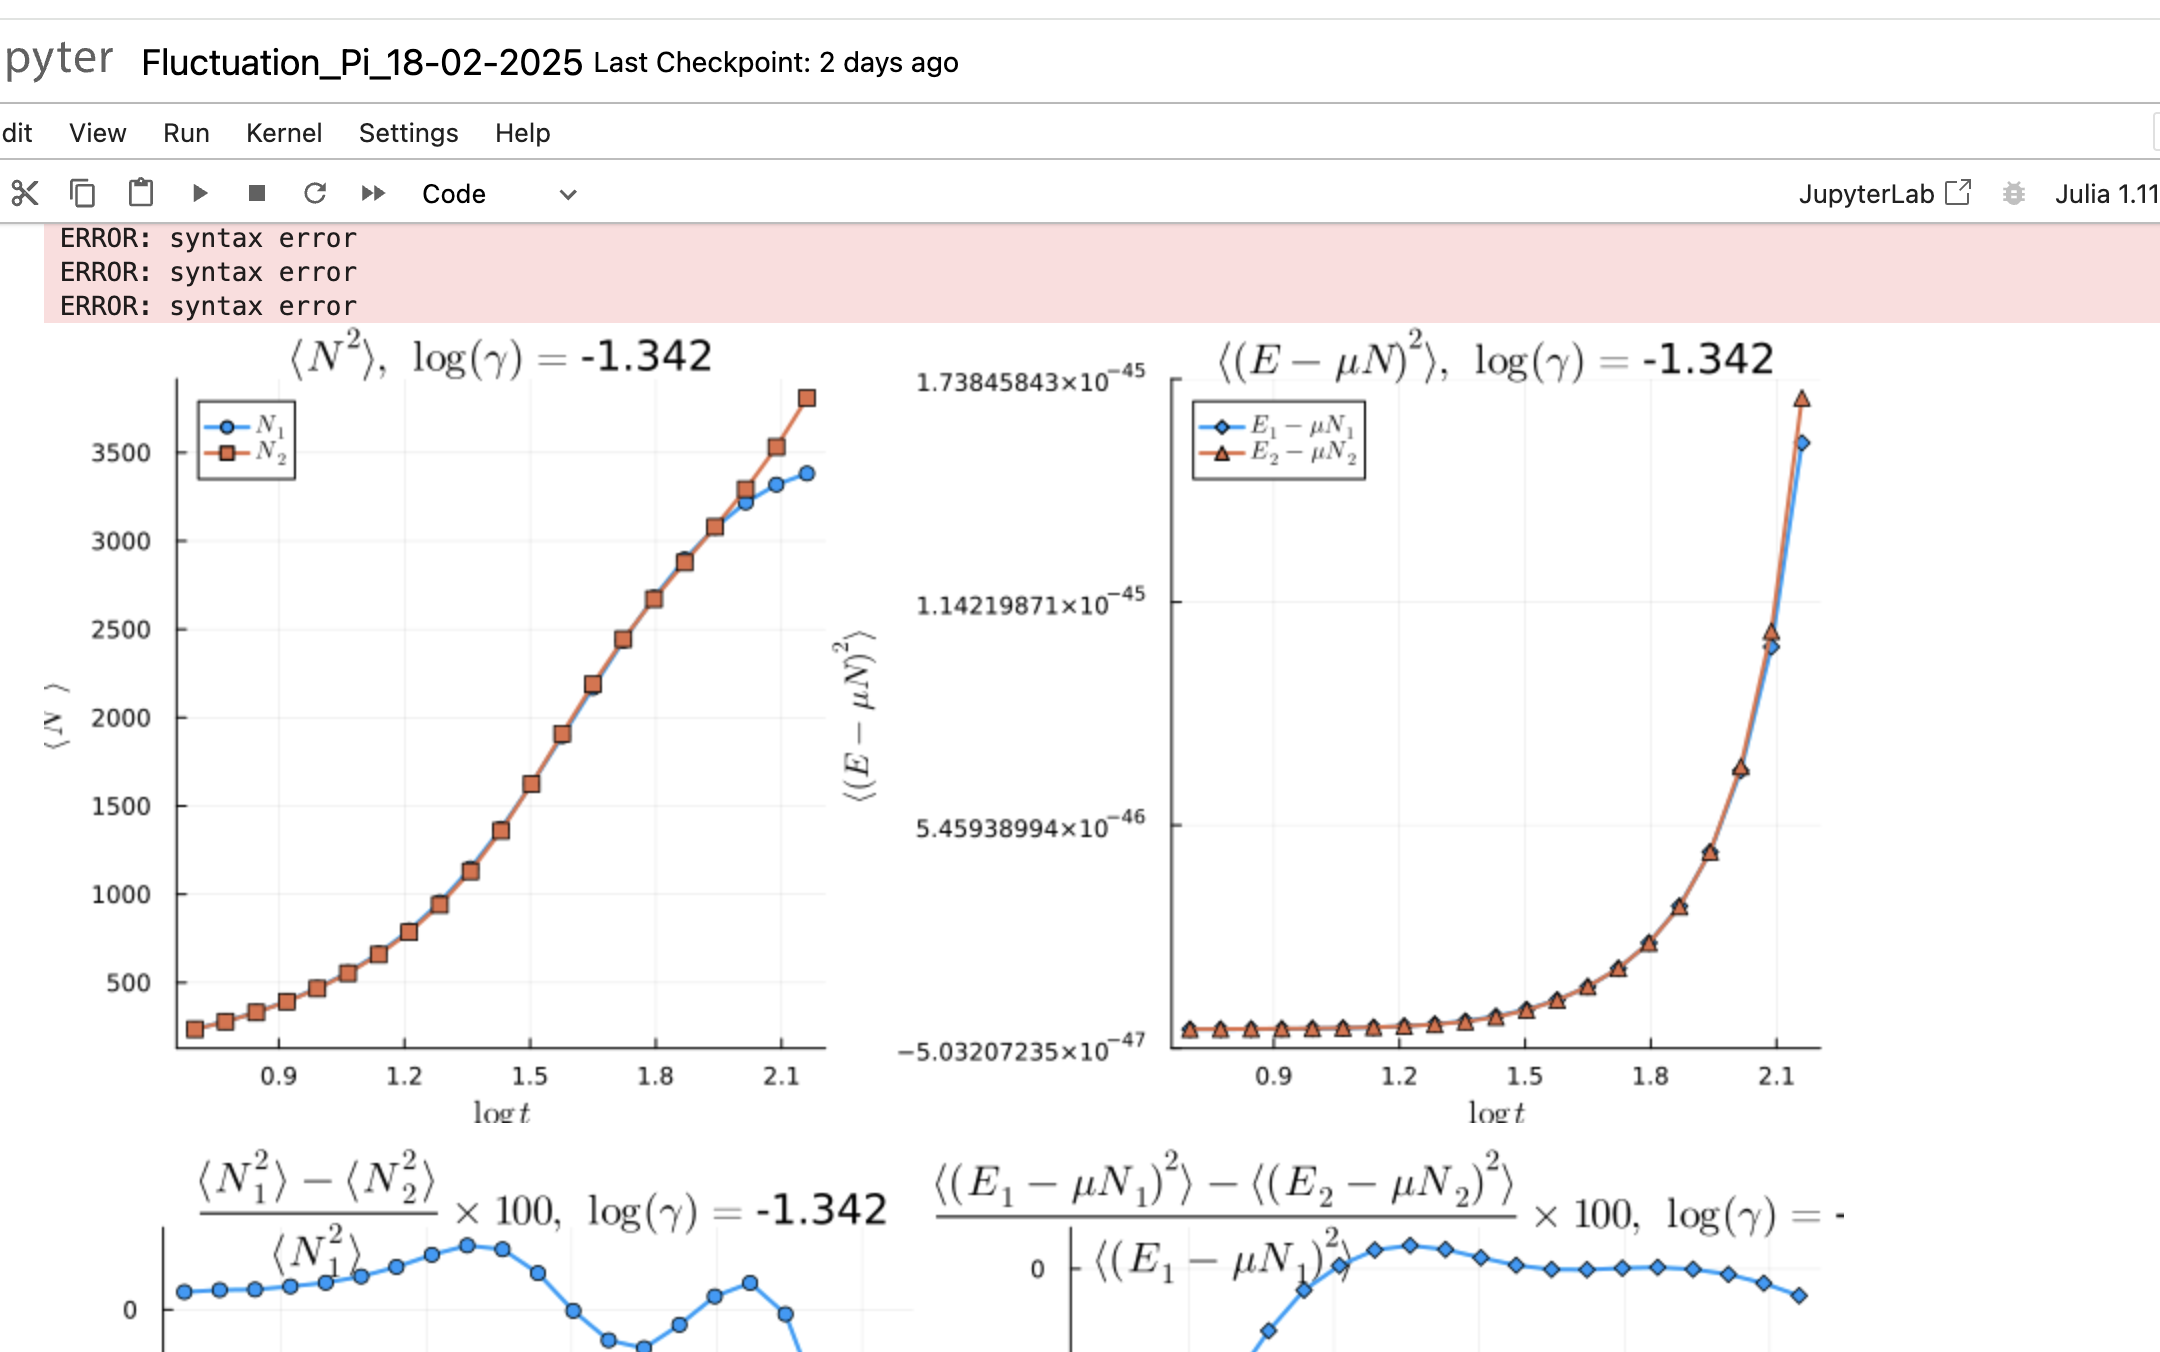
\includegraphics[width=1\textwidth]{Figures/test}

%\begin{aff}
%Donc une a l'ordre un en $\delta \theta (\operator{A}^{(0)})^{-1} %\operator{V}$ 

%\begin{eqnarray*}
%	\langle \delta \Pi ( \theta) \delta \Pi ( \theta') \rangle & = &  ( (\Pi^c_s - \Pi^c)\Pi^c/\Pi^c_s ) ( \theta ) \delta_{\theta, \theta'}/\delta \theta + \mathscr{F}(\theta , \theta' ) ,	
%\end{eqnarray*}

%avec 

%\begin{eqnarray*}
%	\mathscr{F}(\theta , \theta' ) & = & \left [ (\Pi^c_s - \Pi^c )( \theta)  +  (\Pi^c_s - \Pi^c ) ( \theta' )\right ] \frac{\Pi^c}{\Pi^c_s}(\theta)\frac{\Pi^c}{\Pi^c_s}(\theta') \frac{ \Delta( \theta'- \theta )}{ 2 \pi }\\
%	&&  - \left [ (\Pi^c_s - \Pi^c )( \theta)   (\Pi^c_s - \Pi^c ) ( \theta' )\right ] \frac{\Pi^c}{\Pi^c_s}(\theta)\frac{\Pi^c}{\Pi^c_s}(\theta')\int d\theta'' \left (   \frac{ \Pi^c/\Pi^c_s}{\Pi^c_s - \Pi^c} \right )(\theta'') \frac{\Delta(\theta''- \theta)}{2 \pi}\frac{\Delta(\theta''- \theta')}{2 \pi}  	
%\end{eqnarray*}
%\end{aff}



 








\subsection{Excitations élémentaires à température nulle}
%Nous allons d'abord considérer les excitations au-dessus du vide physique dans le secteur de charge physique nulle (c'est-à-dire les excitations où le nombre de particules \( N \) dans l'état excité est identique au nombre de particules dans l'état fondamental). Nous commencerons par des conditions aux limites périodiques (2.13).

L'état fondamental est décrit par un ensemble particulier d'entiers \( n_j \), voir (2.26) et (3.2). Tous les autres ensembles de \( n_j \) (avec la contrainte que \( n_j \neq n_k \)) correspondent à des états excités. Cela constitue une description complète de tous les états excités. Ces excitations sont obtenues en supprimant un certain nombre de particules ayant des moments \( -q < \lambda < q \) de la distribution du vide (c'est-à-dire en créant des trous avec des moments \( \lambda_h \)) et en ajoutant un nombre égal de particules ayant des moments \( \lambda_p > q \).

Nous allons d'abord construire l'état dans lequel une particule de moment \( \lambda_p > q \) diffuse avec un trou de moment \( -q < \lambda_h < q \). La présence simultanée de la particule et du trou modifie les valeurs permises des moments des particules du vide : \( \lambda_j \to \tilde{\lambda}_j \), de sorte que les équations de Bethe pour les particules du vide sont réécrites comme suit.

En soustrayant cette contribution de la distribution du vide (3.2) et en tenant compte du fait que \( \lambda_j - \lambda_j' = \mathcal{O}(1/L) \) et que \( \theta( \lambda + \Delta) - \theta(\lambda) = \mathcal{O}(\Delta) \), on obtient :

En utilisant les équations (2.31), (3.5) et (3.7), on obtient :

On introduit maintenant la "fonction de décalage" \( F \) :

Dans la limite thermodynamique, on peut remplacer la somme dans (4.3) par une intégrale, ce qui donne :
Ainsi, nous sommes en mesure de décrire la polarisation du vide causée par une particule et un trou. Cela permet le calcul des grandeurs observables (énergie, momenta, et matrice de diffusion) pour les excitations au-dessus de l'état fondamental. Ces grandeurs observables sont obtenues en ajoutant les contributions de la polarisation du vide aux quantités "pures" correspondantes. Nous commençons par calculer l'énergie observable \( E \), qui est égale à l'énergie de l'état excité moins l'énergie de l'état fondamental :\\

où \( E_0(\lambda) = \lambda2 - h \). De même, on a pour le moment observable (le moment "pur" est simplement égal à $\lambda$) :

Toutes les excitations dans le secteur à charge nulle peuvent être construites comme un état de diffusion constitué de nombres égaux de particules et de trous. L'énergie et le moment de ces excitations sont égaux à la somme des énergies et des moments des particules et des trous individuels. L'excitation à une particule et un trou construite ci-dessus est un état à deux corps. Dans l'ensemble canonique grand, nous pouvons changer le nombre de particules. Construisons une excitation à une particule avec énergie :

et le moment \( k(p) \) égal à :

(voir (3.7)). Il s'agit d'une excitation topologique (nous devons changer les conditions aux frontières en antipériodiques). La valeur \( \lambda_p \) doit être en dehors de la sphère de Fermi, \( |\lambda_p| > q \), \( \text{Im} \, \lambda_p = 0 \). On peut également construire une autre excitation topologique (trou élémentaire) avec une énergie égale à \( -e(h) \) et un moment égal à :

où \( -q < \lambda < g \). Cela montre que les états excités dans le secteur neutre construits ci-dessus sont constitués de deux excitations élémentaires (comparer les formules (4.19) et (4.20) avec (4.16)). Pour construire ces excitations topologiques, il faut changer les conditions aux frontières pour qu'elles soient antipériodiques lors de l'introduction d'une excitation.

Cette excitation topologique a une nature fermionique. Pour les bosons implacables, cela est explicitement montré dans l'Appendice 1. Ainsi, nous allons introduire une autre particule dans l'état fondamental et changer les conditions aux frontières.
Dans l'état excité, il y a \( N + 1 \) particules avec des moments \( \tilde{\lambda}_j; j = 1, \dots, N + 1 \). Les équations de Bethe correspondantes sont :

L'état excité est caractérisé par l'ensemble de \( N + 1 \) nombres \( \{ n_j, j = 1, \dots, N + 1 \} \); les \( N \) premiers nombres correspondent à l'état fondamental (2.26). Notons \( \lambda_{N+1} \) par \( \lambda_p \). Il est commode d'introduire une fonction de décalage \( F \) similaire à celle de (4.4) :

Dans la limite thermodynamique, la fonction de décalage satisfait l'équation intégrale suivante :

où \( |\lambda_p | > q \). La fonction \( F(\mu|\lambda) \) est définie pour \( |\mu| < q \); cependant, à l'aide de l'équation (4.25), \( F \) peut être prolongée analytiquement sur tout l'axe réel.

Avec l'aide de la fonction de décalage, nous pouvons calculer les quantités observables dans la limite thermodynamique (énergie, moment et matrice de diffusion). La fonction de décalage décrit le nuage de particules virtuelles qui entoure la particule \( p \) ou, en d'autres termes, la polarisation du vide due à la particule nue \( p \). Des calculs similaires à ceux du début de cette section montrent que l'énergie d'une particule est \( \varepsilon(\lambda_p) \) (voir (4.9)) et que le moment est donné par (4.19).

Une excitation de "trou" peut être traitée de manière similaire. Le nombre de particules dans cette excitation est égal à \( N - 1 \) et la charge observable est égale à \( -1 \). La fonction d'onde \( X_N \) doit à nouveau être antiperiodique. Cet état est caractérisé par l'ensemble de nombres entiers \( \{n_j\} \) obtenu en éliminant un nombre de l'ensemble du vide. La fonction de décalage satisfait l'équation

où \( | \lambda_h | < q \) est le moment de la particule nue du trou. Avec l'aide de cette fonction, l'énergie et le moment peuvent être obtenus :


Cette fonction peut être remplacée par \( -k_h(\lambda_h) \) trouvé dans (4.19).
Les excitations arbitraires sont construites à partir de plusieurs particules et trous.
L'énergie et le moment de telles excitations sont simplement la somme des contributions des excitations élémentaires individuelles. Ainsi, l'énergie et le moment sont donnés par :


La matrice de diffusion à plusieurs corps est simplement le produit des matrices de diffusion à deux corps. D'abord, la matrice de diffusion pour deux particules sera évaluée. L'ajout de deux particules (\( \lambda_2 > \lambda_1 > q \)) au vide déplace les valeurs des moments des particules du vide : \( \lambda_j \rightarrow \tilde{\tilde{\lambda}}_j \) (pour \( j = 1, \ldots, N \)). La fonction de décalage

est égale à la somme des fonctions de décalage à une particule données par (4.25) :

Maintenant, considérons la matrice de diffusion de deux particules possédant des moments \( \lambda_1 \) et \( \lambda_2 \) avec \( \lambda_2 > \lambda_1 > q \), comme ci-dessus. Dans ce cas, la matrice de diffusion est simplement un facteur numérique de module unitaire ; ainsi, elle peut être écrite comme


Le phase \( \delta \) est réelle et est donnée par


où \( \varphi_2 \) est la phase complète que la deuxième particule acquiert lorsqu'elle traverse l'ensemble de la boîte dans le cas où la première particule est absente :

La phase \( \varphi_{21} \) est la phase complète que la deuxième particule acquiert lorsqu'elle traverse l'ensemble de la boîte en présence de la première :

En utilisant les équations (4.34) et (4.35), la phase de diffusion est donnée par

En changeant la somme en une intégrale dans la limite thermodynamique et en utilisant (4.31), on obtient

et à partir de (4.25)

Ainsi, la phase de diffusion satisfait l'équation intégrale suivante :

Nous avons démontré que les excitations physiques au-dessus de la mer de Dirac sont obtenues à partir des excitations "nues" au-dessus du vide de Fock \( |0\rangle \) (qui sont décrites par les fonctions d'onde de Bethe) à travers les équations de "dressing". Ces équations linéaires intégrales de dressing sont des équations universelles. Pour le voir, il suffit de comparer les équations de dressing pour l'énergie (4.9), la phase de diffusion (4.39) et la densité (3.7). Les équations de dressing sont également très utiles pour l'étude des fonctions de corrélation et des corrections de taille finie, comme nous le verrons dans les sections suivantes.

La diffusion de deux trous ayant des momenta nues \( \lambda_1 \) et \( \lambda_2 \), avec \( -q \leq \lambda_{1, 2} \leq q \), est également égale à \( \exp\left(i \varphi(\lambda_2, \lambda_1)\right) \) où \( \varphi \) est défini par (4.39). La matrice de diffusion de la particule \( \lambda_p \) avec le trou \( \lambda_h \) est égale à


La matrice de diffusion de plusieurs particules est égale au produit des matrices de diffusion à deux particules.

Il convient également de mentionner que les structures d'excitation d'autres modèles (antiferromagnétique XXZ de Heisenberg et modèle de sine-Gordon) sont très similaires. L'énergie, le moment et la matrice de diffusion sont évalués de la même manière.







